\chapter{Resultados}
\label{chap:res}

Como se indica en el cap\'itulo \ref{chap:cap2}, la obtenci\'on de un grafo a partir de una imagen, es un proceso complejo. Las im\'agenes analizadas en este trabajo son aquellas en las que fue posible realizar el procedimiento de esqueletonizaci\'on, obteniendo un resultado que manten\'ia la topolog\'ia de la estructura original. Lo anterior no es un estando que pueda garantizarse para toda imagen. 


Los resultados que se presentan a continuaci\'on se separan entre tablas y figuras. Las tablas de resultados se encuentran dividas en 2 secciones dado el n\'umero de columnas. La primera secci\'on agrupa las m\'etricas y medidas indicadas en la secci\'on \ref{sec:metricasymedidas}. La segunda secci\'on muestra los porcentajes de cobertura y correctitud de los filamentos propuestos con respecto al {\it ground truth}. Es importante aclarar que aun cuando en la mayor\'ia de la tablas de resultados la columna `` \% Cobertura de Aristas'' es del 100\%, este no es siempre el caso para el algoritmo Phil, ya que no tiene como restricci\'on estricta garantizar la cobertura de cada arista del grafo, a diferencia de DeFiNe.

En cuanto a las figuras, el enfoque se dirige a presentar los resultados de DeFiNe y Phil, con \'enfasis en los filamentos correctamente encontrados por uno de los algoritmos que el otro no haya podido individualizar. Cabe aclarar que el resultado gr\'afico al ejecutar DeFiNe realiza una rotaci\'on de 90\textdegree en sentido contrarreloj adem\'as de invertir el eje vertical. Ambas modificaciones han sido corregidas con el prop\'osito de comparar los resultados entre DeFiNe, Phil y la individualizaci\'on de filamentos realizada por el experto.


En las mediciones del algoritmo {\it Phil}, se muestra el promedio de las 5 iteraciones con diferentes semillas que se realizaron. El detalle de cada iteraci\'on se encuentra en el ap\'endice \ref{chap:apendice}.
Las ejecuciones de DeFiNe y Phil fueron realizadas en un computador con un procesador {\tt Intel i5-7200U} de 4 n\'ucleos, 8GB de RAM y un disco de estado s\'lido, bajo el sistema operativo {\tt Fedora 31}.

\section{Im\'agenes Sint\'eticas}

Los resultados de la figura \ref{fig:synth-QFS-7} indicados en la tabla \ref{tab:synth-QFS-7-Results} muestran un mejor desempe\~no de DeFiNe, que encuentra un filamento m\'as que Phil con respecto a la individualizaci\'on realizada por el experto.

\begin{table}[h]
    \centering
    \begin{tabular}{|c|c|c|c|c|c|c|c|c|c|c|}
    \hline
        Algoritmo & VI & TP & FP &TN &FN & Rand	& Jaccard &	Precision &	Recall &	F1 \\ \hline
        Define 30° & 1.3859 & 5 & 6 & 55 & 12 & 0.7692  & 0.2173 & 0.4545 & 0.2941 & 0.3571\\
        Define 60° & 1.5677 & 4 & 7 & 47 & 8  & 0.7727  & 0.2105  & 0.3636  & 0.3333 & 0.3478\\ 
        Phil & 1.6360 & 10.8 & 10.4 & 104.8 & 28 & 0.7646 & 0.2484 & 0.5142 & 0.3289 & 0.3919\\
        \hline
    \end{tabular}
    \caption{Resultados de individualizaci\'on de filamentos para figura \ref{fig:synth-QFS-7}. El valor m\'aximo de VI en este caso es de 2.397895, ya que el tama\~no del {\it data set} es de 11 aristas. El n\'umero de filamentos en el {\it ground truth} es 6.}
    \label{tab:synth-QFS-7-Results}
\end{table}
\addtocounter{table}{-1}
\begin{table}[h]
    \centering
    \begin{tabular}{|c|c|c|c|c|c|c|}
    \hline
         & \multirow{4}{2cm}{\centering \% Cobertura de Aristas} & \multirow{4}{2cm}{Filamentos Propuestos} & \multirow{4}{2cm}{Filamentos Correctos} & \multirow{4}{2.5cm}{\% Correctos vs Propuestos} & \multirow{4}{2.5cm}{\centering \% Correctos vs {\it Ground Truth}} & \multirow{4}{1.2cm}{\centering Tiempo [seg]} \\
         &  &  &  & & &  \\
        Algoritmo &  &  &  & & &  \\
        &  &  &  & & &  \\ \hline
        Define 30° & 100 & 6 & 4 & 66.6667 & 66.6667 & 2.3128\\
        Define 60° & 100 & 5 & 4 & 80 & 66.6667 & 2.3380\\ 
        Phil & 100 & 6.2 & 3 & 49.1428 & 50  & 0.3569\\
        \hline
    \end{tabular}
    \caption{Resultados ({\it Continuaci\'on}) de individualizaci\'on de filamentos para figura \ref{fig:synth-QFS-7}. El n\'umero de filamentos en el {\it ground truth} es 6.}
    %\label{tab:synth-QFS-7-Results2}
\end{table}


\begin{table}[h]
    \centering
    \begin{tabular}{|c|c|c|c|c|c|c|c|c|c|c|}
    \hline
        Algoritmo & VI & TP & FP &TN &FN & Rand	& Jaccard &	Precision &	Recall &	F1 \\ \hline
        Define 30° & 1.8102 & 6 & 14 & 156  & 34 & 0.7714 & 0.1111  & 0.3 & 0.15 & 0.2\\
        Define 60° & 2.2890 & 19 & 52 & 200 & 54 & 0.6738 & 0.152 & 0.2676  & 0.2602  & 0.2638\\ 
        Phil & 2.2164 & 22.8 & 40 & 240.4 & 61.4 & 0.7227 & 0.1838 & 0.3607 & 0.2724 & 0.3100\\
        \hline
    \end{tabular}
    \caption{Resultados de individualizaci\'on de filamentos para figura \ref{fig:synth-Define-1b}.El valor m\'aximo de VI en este caso es de 3.044522, ya que el tama\~no del {\it data set} es de 17 aristas. El n\'umero de filamentos en el {\it ground truth} es 5.}
    \label{tab:synth-Define-1b}
\end{table}
\addtocounter{table}{-1}
\begin{table}[h]
    \centering
    \begin{tabular}{|c|c|c|c|c|c|c|}
    \hline
         & \multirow{4}{2cm}{\centering \% Cobertura de Aristas} & \multirow{4}{2cm}{Filamentos Propuestos} & \multirow{4}{2cm}{Filamentos Correctos} & \multirow{4}{2.5cm}{\% Correctos vs Propuestos} & \multirow{4}{2.5cm}{\centering \% Correctos vs {\it Ground Truth}} & \multirow{4}{1.2cm}{\centering Tiempo [seg]} \\
         &  &  &  & & &  \\
        Algoritmo &  &  &  & & &  \\
        &  &  &  & & &  \\ \hline
        Define 30° & 100 & 11 & 2 & 18.1818 & 40 & 2.8275\\
        Define 60° & 100 & 7 & 2 & 28.5714 & 40 & 3.6597\\ 
        Phil & 100 & 9.2 & 3 & 32.6667 & 60 & 0.5071\\
        \hline
    \end{tabular}
    \caption{Resultados ({\it Continuaci\'on}) de individualizaci\'on de filamentos para figura \ref{fig:synth-Define-1b}. El n\'umero de filamentos en el {\it ground truth} es 5.}
    %\label{tab:synth-QFS-7-Results2}
\end{table}

\section{Im\'agenes Reales}

%recordar que define es base de BFS-Overlap-pairwise-total-
% recordarr que son 5 iteraciones y se estan promediando los resultados, conectar con la columna cobertura 



\subsection{Microt\'ubulos}

%Valor m\'ax de VI para \ref{tab:SpinningMarchantiaResults1} es 3.4965.
%N\'umero de filamentos en el {\it Ground Truth} de la figura SpinningMarchanria es 12.
%Define y Phil presentan una propuesta de filamento para el ....

\begin{figure*}[h!]
    \centering
    \begin{subfigure}[t]{0.49\textwidth}
        \centering
        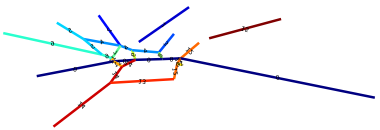
\includegraphics[scale=0.6]{resultImages/SpinningMarchantia-Define30.png}
        \caption{Individualizaci\'on mediante DeFiNe con 30\textdegree}
        \label{fig:SpinningMarchantiaResults-define30}
    \end{subfigure}%
    ~ 
    \begin{subfigure}[t]{0.49\textwidth}
        \centering
        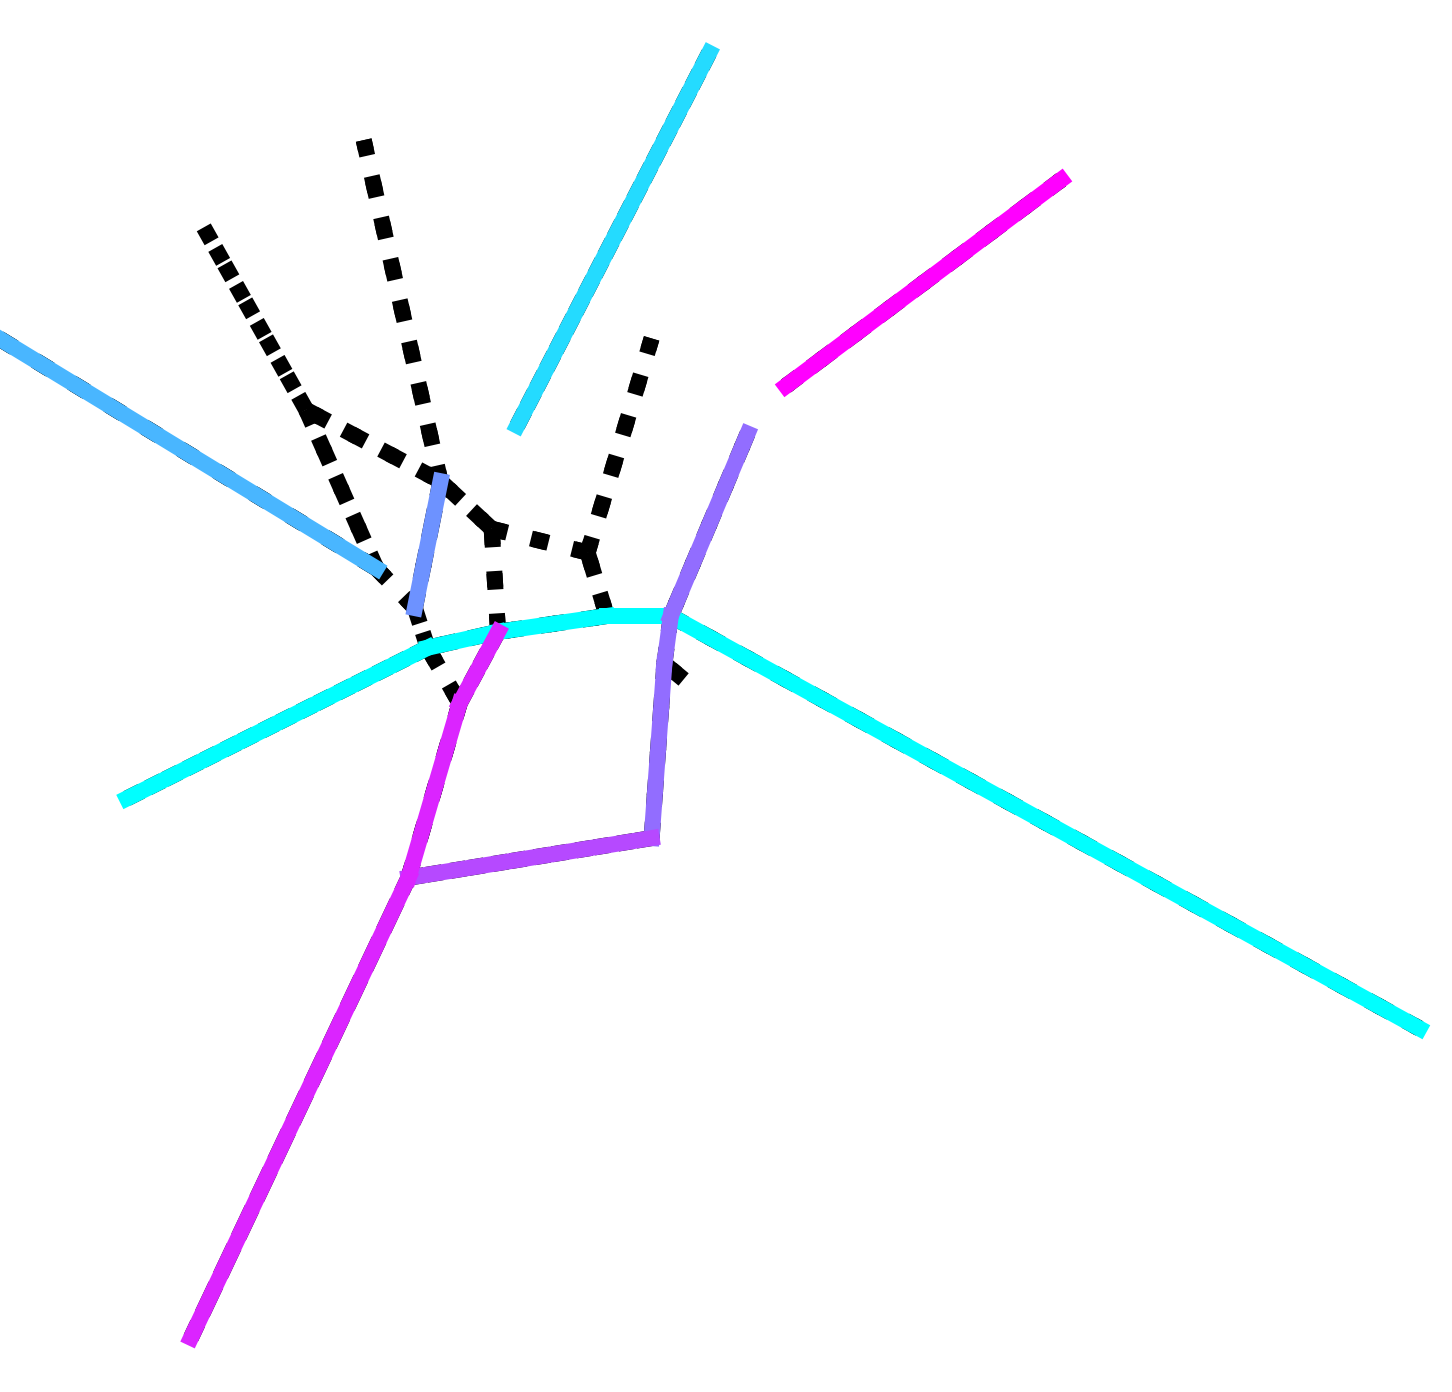
\includegraphics[height=1.5in]{resultImages/50-ROIs-Spinning-Marchantia-DeFiNeExactMatch-30.png}
        \caption{Filamentos correctamente individualizados por DeFiNe con 30\textdegree identificados con colores}
        \label{fig:SpinningMarchantiaResults-define30Exact}
    \end{subfigure}
    \vskip\baselineskip
    
    \begin{subfigure}[t]{0.49\textwidth}
        \centering
        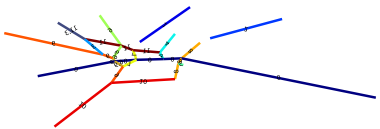
\includegraphics[scale=0.6]{resultImages/SpinningMarchantia-Define60.png}
        \caption{Individualizaci\'on mediante DeFiNe con 60\textdegree}
        \label{fig:SpinningMarchantiaResults-define60}
    \end{subfigure}
    ~ 
    \begin{subfigure}[t]{0.49\textwidth}
        \centering
        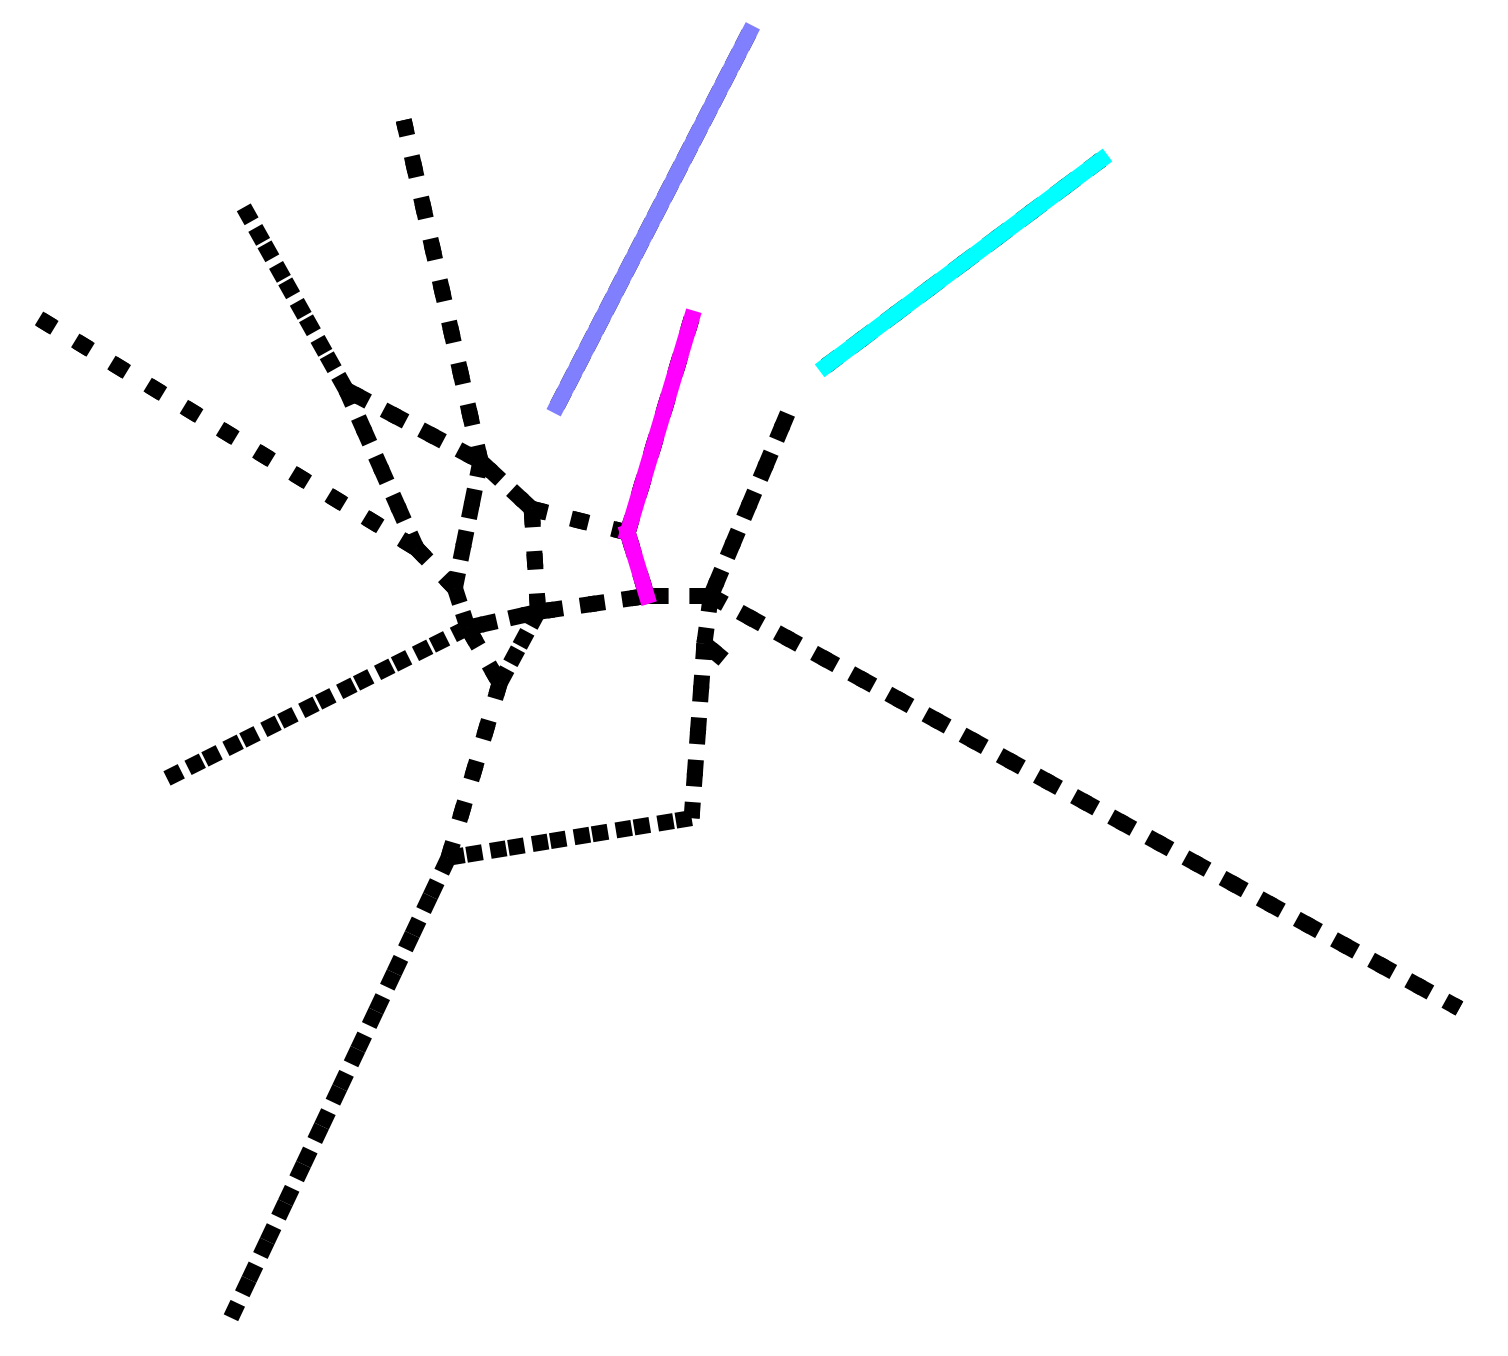
\includegraphics[height=1.5in]{resultImages/50-ROIs-Spinning-Marchantia-DeFiNeExactMatch-60.png}
        \caption{Filamentos correctamente individualizados por DeFiNe con 60\textdegree identificados con colores}
        \label{fig:SpinningMarchantiaResults-define60Exact}
    \end{subfigure}
    \vskip\baselineskip
    
    \begin{subfigure}[t]{0.49\textwidth}
        \centering
        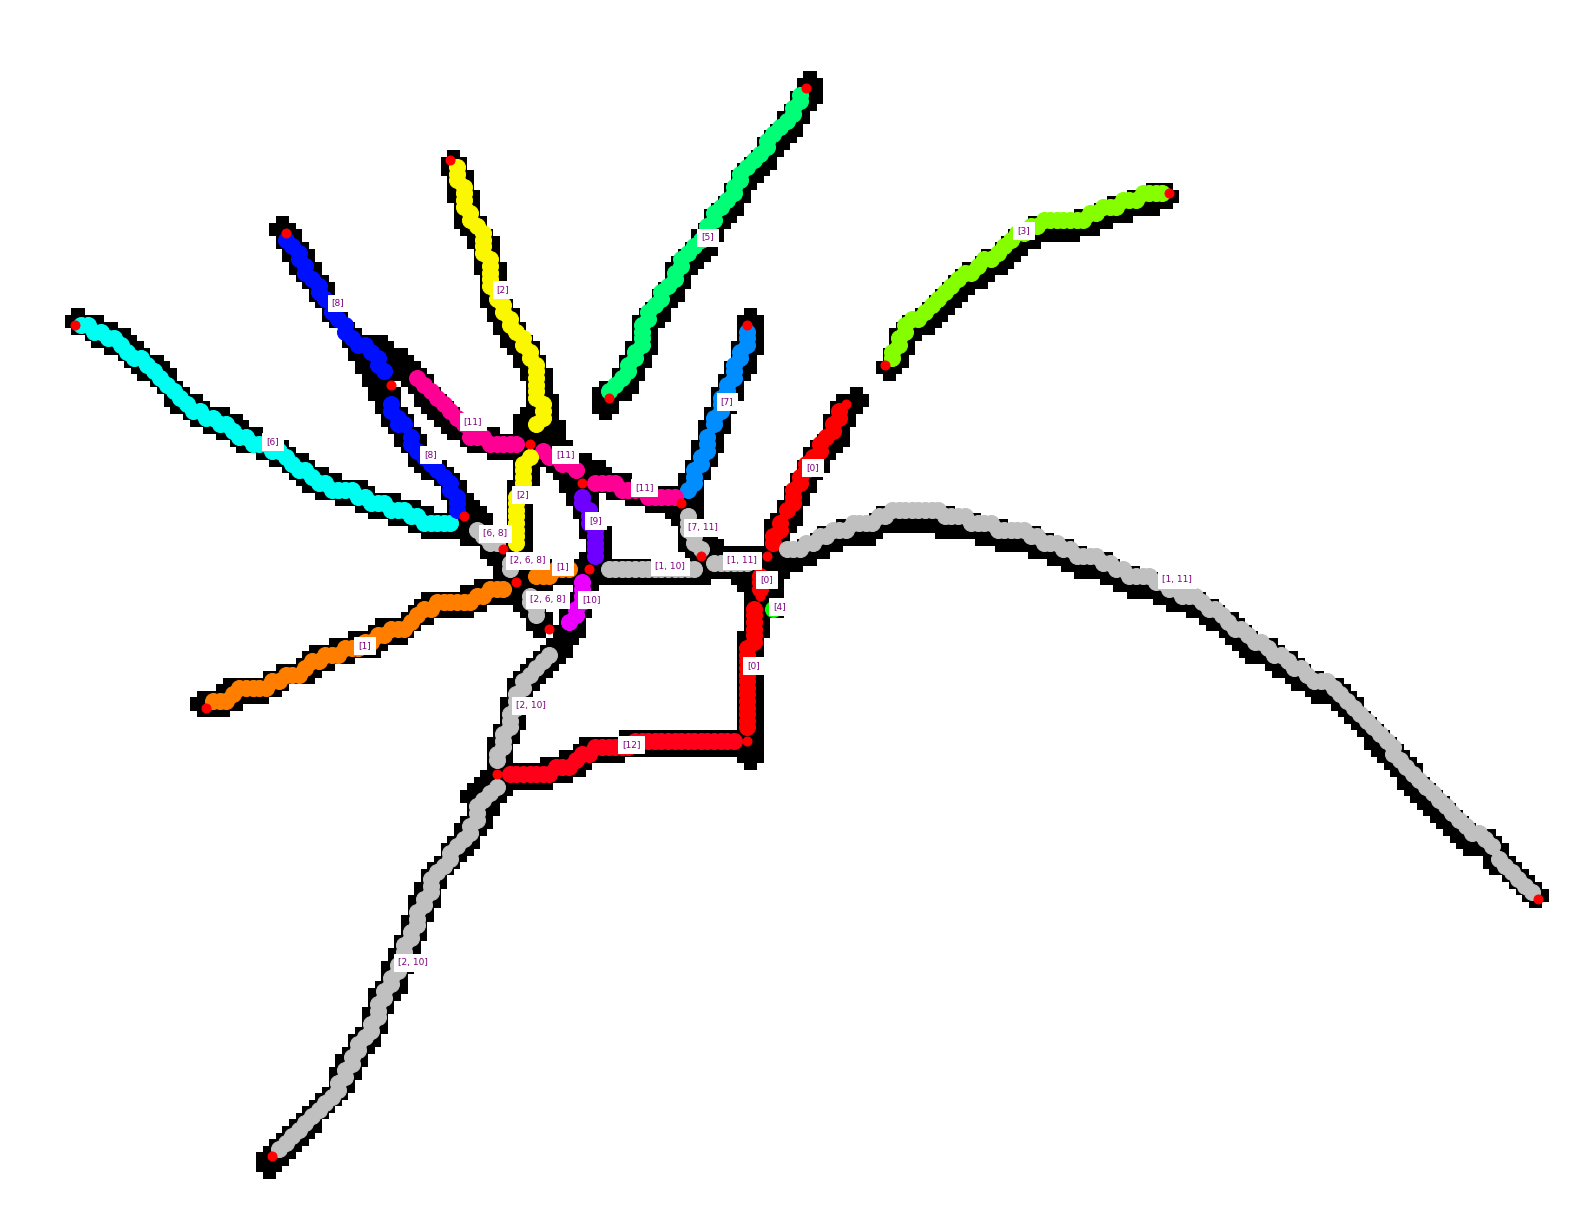
\includegraphics[height=1.5in]{resultImages/50-ROIs-Spinning-Marchantia-phil-s0-v05-antLabeled.png}
        \caption{Mejor resultado de individualizaci\'on de filamentos de Phil}
        \label{SpinningMarchantiaResults-bestPhil}
    \end{subfigure}
    ~
    \begin{subfigure}[t]{0.49\textwidth}
        \centering
        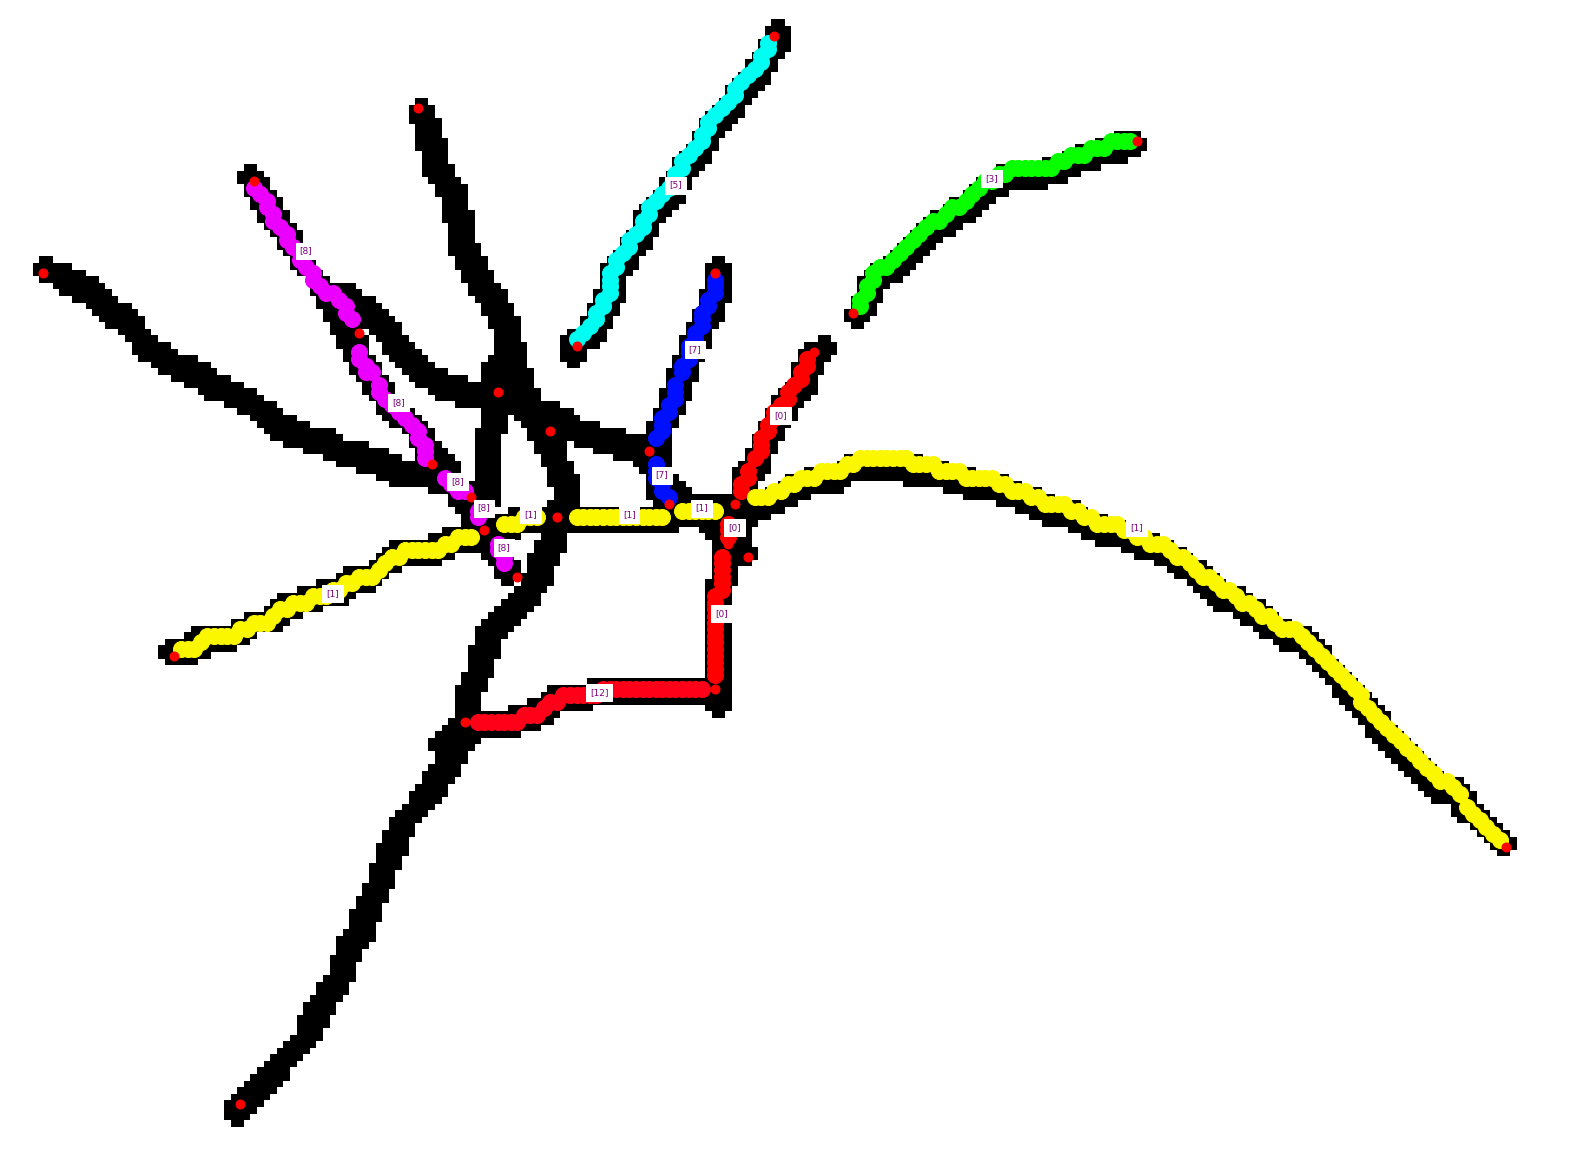
\includegraphics[height=1.5in]{resultImages/50-ROIs-Spinning-Marchantia-phil-s0-v05-exactMatch-antLabeled.png}
        \caption{Individualizaci\'on de filamentos correctos del mejor resultado de Phil}
        \label{fig:SpinningMarchantiaResults-bestPhilExact}
    \end{subfigure}
    \vskip\baselineskip
    
    \begin{subfigure}[t]{0.49\textwidth}
        \centering
        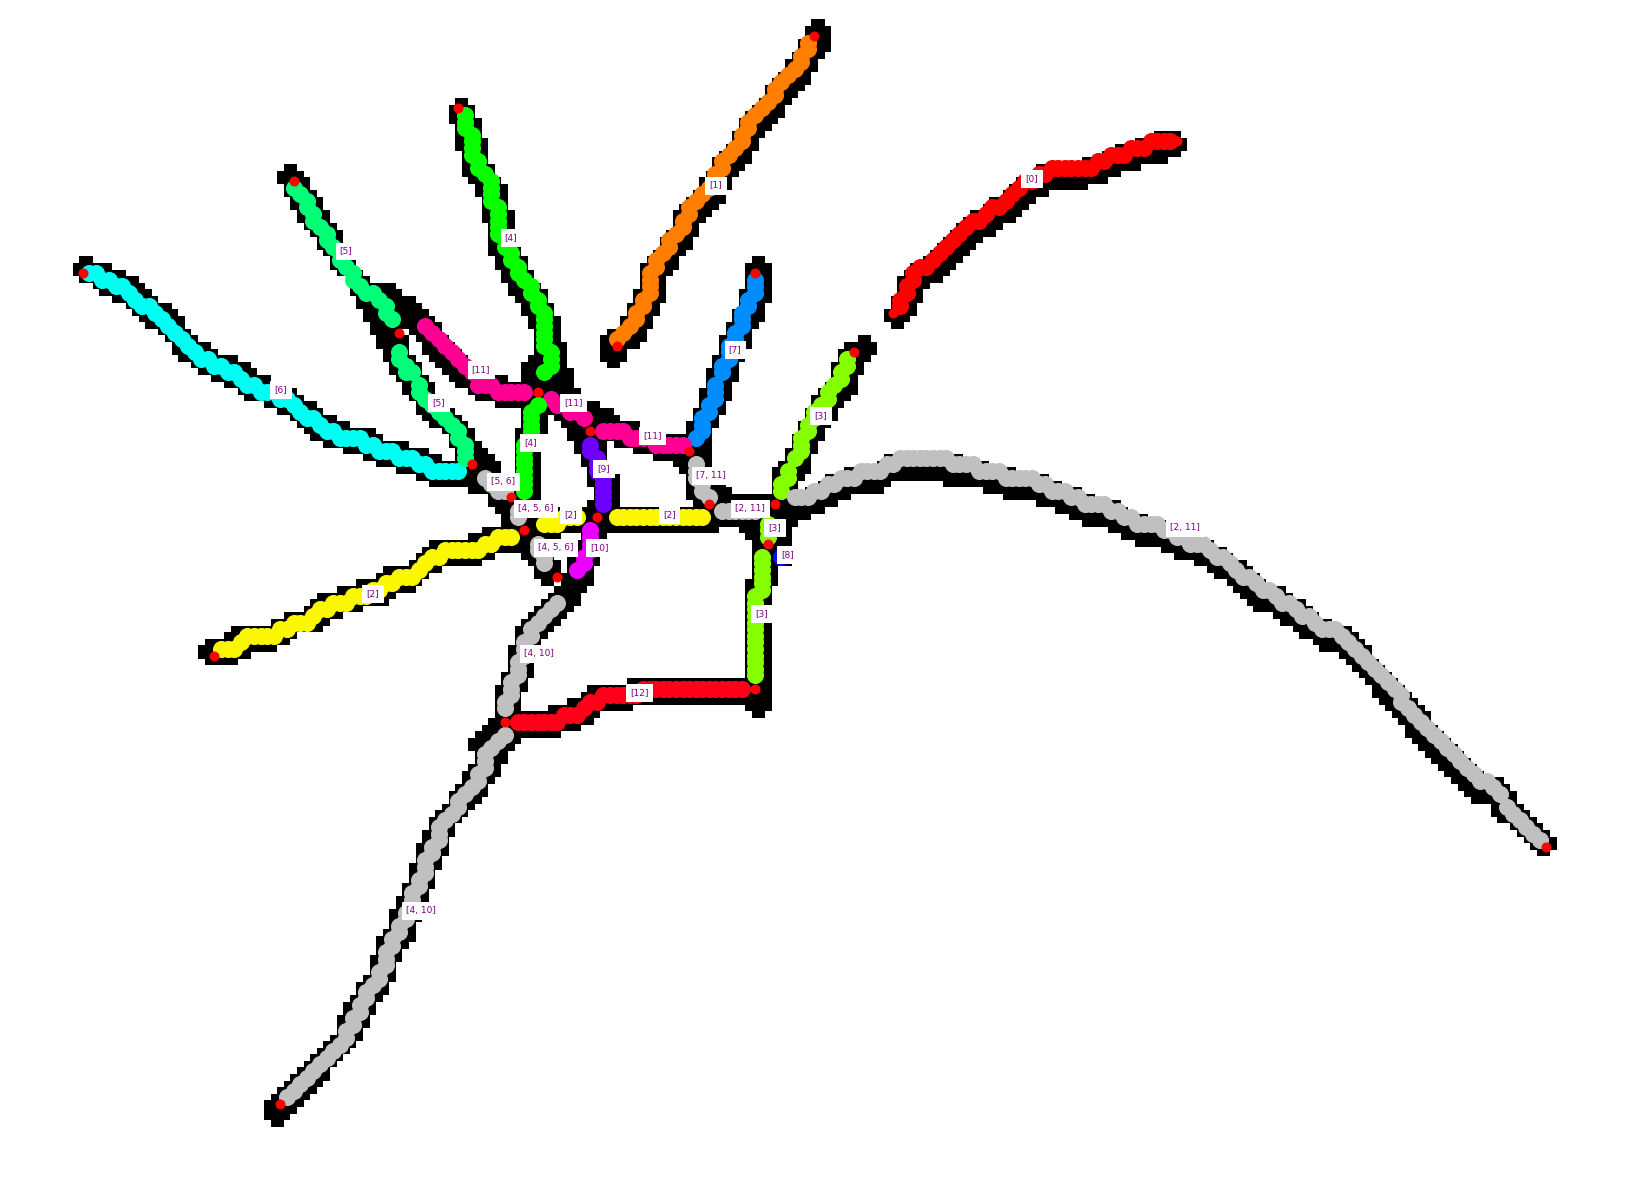
\includegraphics[height=1.5in]{resultImages/50-ROIs-Spinning-Marchantia-phil-s10-v05-antLabeled.png}
        \caption{Peor resultado de individualizaci\'on de filamentos de Phil}
        \label{SpinningMarchantiaResults-worstPhil}
    \end{subfigure}
    ~ 
    \begin{subfigure}[t]{0.49\textwidth}
        \centering
        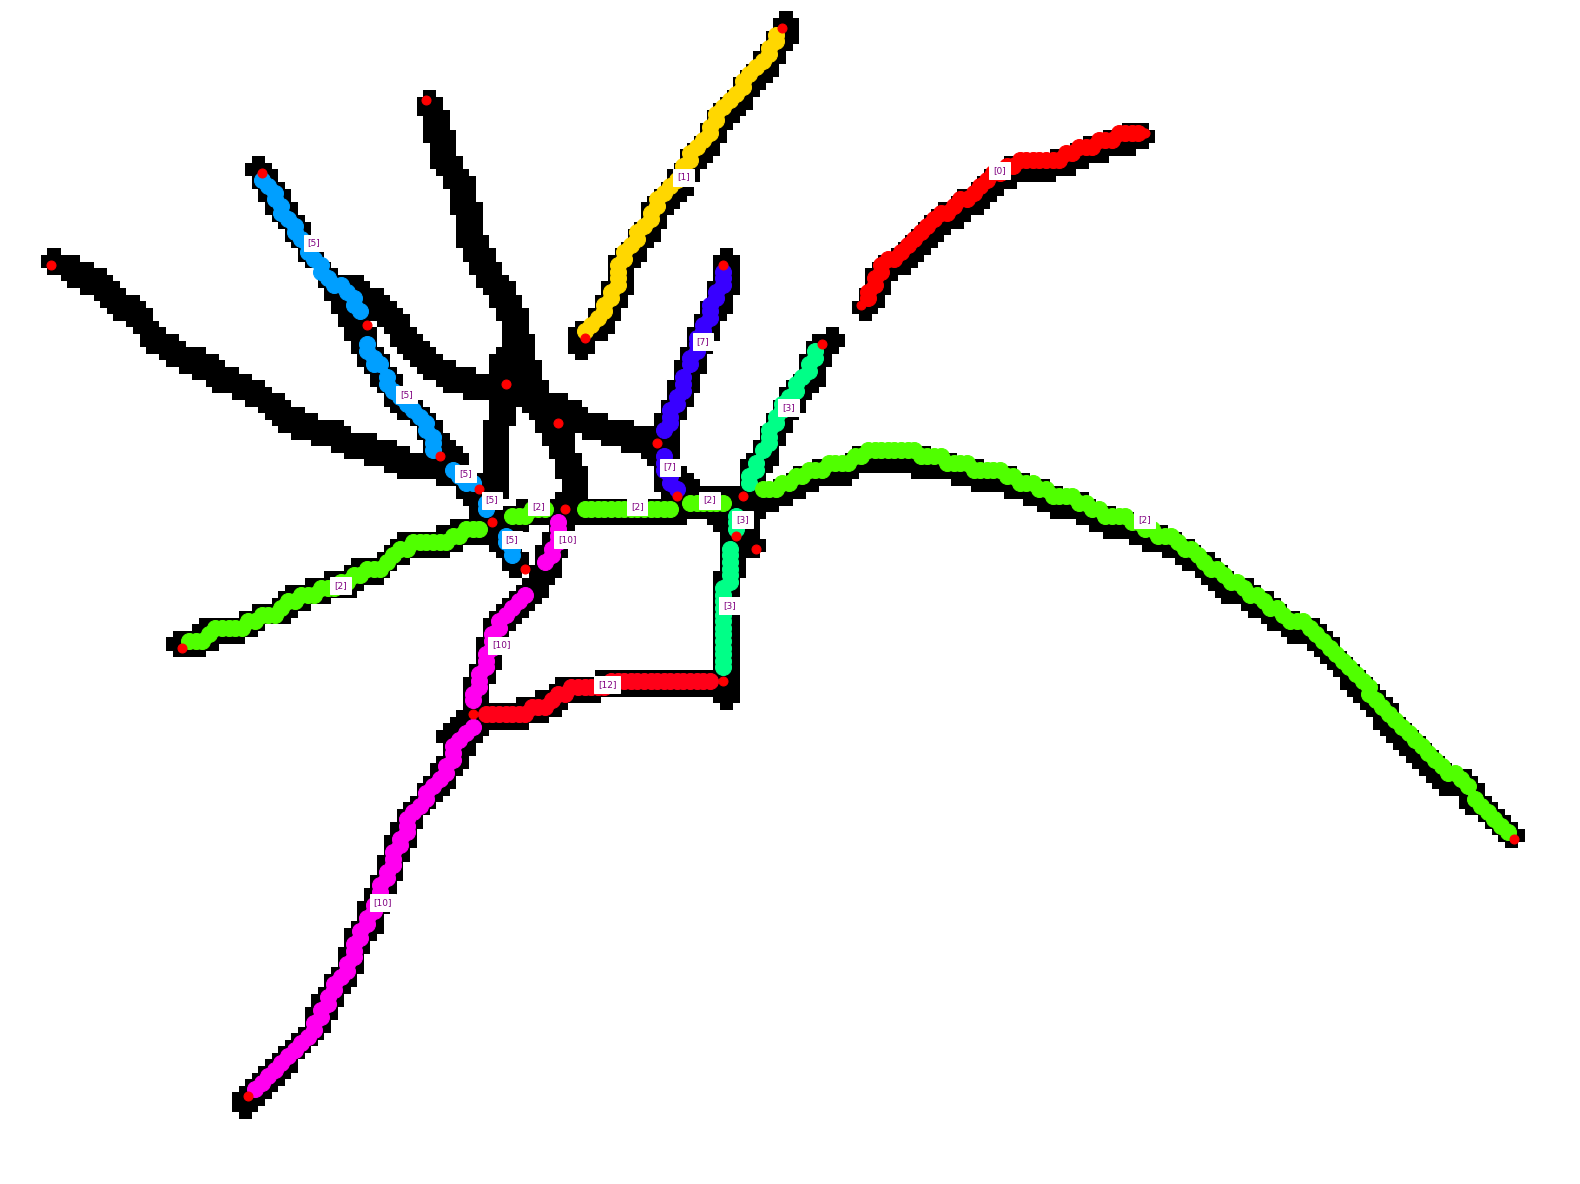
\includegraphics[height=1.5in]{resultImages/50-ROIs-Spinning-Marchantia-phil-s10-v05-exactMatch-antLabeled.png}
        \caption{Individualizaci\'on de filamentos correctos del peor resultado de Phil}
        \label{fig:SpinningMarchantiaResults-worstPhilExact}
    \end{subfigure}
    
    \caption{Individualizaci\'on  de filamentos para la muestra MT-A en la figura \ref{fig:SpinningMarchantia} realizadas con DeFiNe y Phil. Segmentos marcados en negro con y sin discontinuidad representan aristas no asignadas correctamente al filamento correspondiente en el {\it ground truth.}, mientras que los filamentos correctamente identificados se encuentran identificados mediante colores.}
    \label{fig:SpinningMarchantiaResults}
\end{figure*}

\begin{table}[h]
    \centering
    \begin{tabular}{|c|c|c|c|c|c|c|c|c|c|c|}
    \hline
        Algoritmo & VI & TP & FP &TN &FN & Rand	& Jaccard &	Precision &	Recall &	F1 \\ \hline
        Define 30° & 0.9696 & 23 & 12 & 465 & 28 & 0.9242 & 0.3650 & 0.6571 & 0.4509  & 0.5348 \\ 
        Define 60° & 2.2870  & 15 & 38 & 523 & 54 & 0.8539 & 0.1401 & 0.2830 & 0.2173 & 0.2459\\
        Phil & 1.8376 & 43 & 54 & 815 & 78 & 0.8666 & 0.2457 & 0.4432 & 0.3553 & 0.3944 \\
        \hline
    \end{tabular}
    \caption{Resultados de individualizaci\'on de filamentos para la muestra MT-A en la figura \ref{fig:SpinningMarchantia}. El valor m\'aximo de VI en este caso es de 3.4965, ya que el tama\~no del {\it data set} es de 29 aristas. El n\'umero de filamentos en el {\it ground truth} es 12.}
    \label{tab:SpinningMarchantiaResults1}
\end{table}
\addtocounter{table}{-1}
\begin{table}[h]
    \centering
    \begin{tabular}{|c|c|c|c|c|c|c|}
    \hline
         & \multirow{4}{2cm}{\centering \% Cobertura de Aristas} & \multirow{4}{2cm}{Filamentos Propuestos} & \multirow{4}{2cm}{Filamentos Correctos} & \multirow{4}{2.5cm}{\% Correctos vs Propuestos} & \multirow{4}{2.5cm}{\centering \% Correctos vs {\it Ground Truth}} & \multirow{4}{1.2cm}{\centering Tiempo [seg]} \\
         &  &  &  & & &  \\
        Algoritmo &  &  &  & & &  \\
        &  &  &  & & &  \\ \hline
        Define 30° & 100 & 16 & 9 & 56.25       & 75          & 4.1087 \\
        Define 60° & 100 & 12 & 5 & 41.6666 & 41.6666 & 5.9999 \\ 
        Phil & 100 & 12 & 7 & 58.3333 & 58.3333 & 0.6558 \\
        \hline
    \end{tabular}
    \caption{Resultados ({\it Continuaci\'on}) de individualizaci\'on de filamentos para la muestra MT-A en la figura \ref{fig:SpinningMarchantia}. El n\'umero de filamentos en el {\it ground truth} es 12.}
    %\label{tab:SpinningMarchantiaResults2}
\end{table}



%Valor m\'ax de VI para \ref{tab:field3t0filtered1} es 3.7612.
%N\'umero de filamentos en el {\it Ground Truth} de la figura field3t0 es 12.
para la muestra MT-B en la
- A pesar de tener el peor valor de VI, Phil obtiene la mayor cantidad de filamentos correctamente individualizados, en todos sus resultados. 
- encuentra el filamentos conformando por las aristas .... en 4 de las 5 iteraciones ejecutadas para obtener el comportamiento promedio. 
- El promedio de Phil tiene valores para TN/FP/TN/FN  mayores -> m\'as recorrido de soluciones?

\begin{figure*}[h!]
    \centering
    \begin{subfigure}[t]{0.49\textwidth}
        \centering
        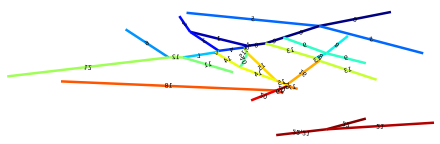
\includegraphics[scale=0.6]{resultImages/field3-t0-2cellBcrop-filtered-Define30.png}
        \caption{Individualizaci\'on mediante DeFiNe con 30\textdegree}
        \label{fig:field3t0filtered1Results-define30}
    \end{subfigure}%
    ~
    \begin{subfigure}[t]{0.49\textwidth}
        \centering
        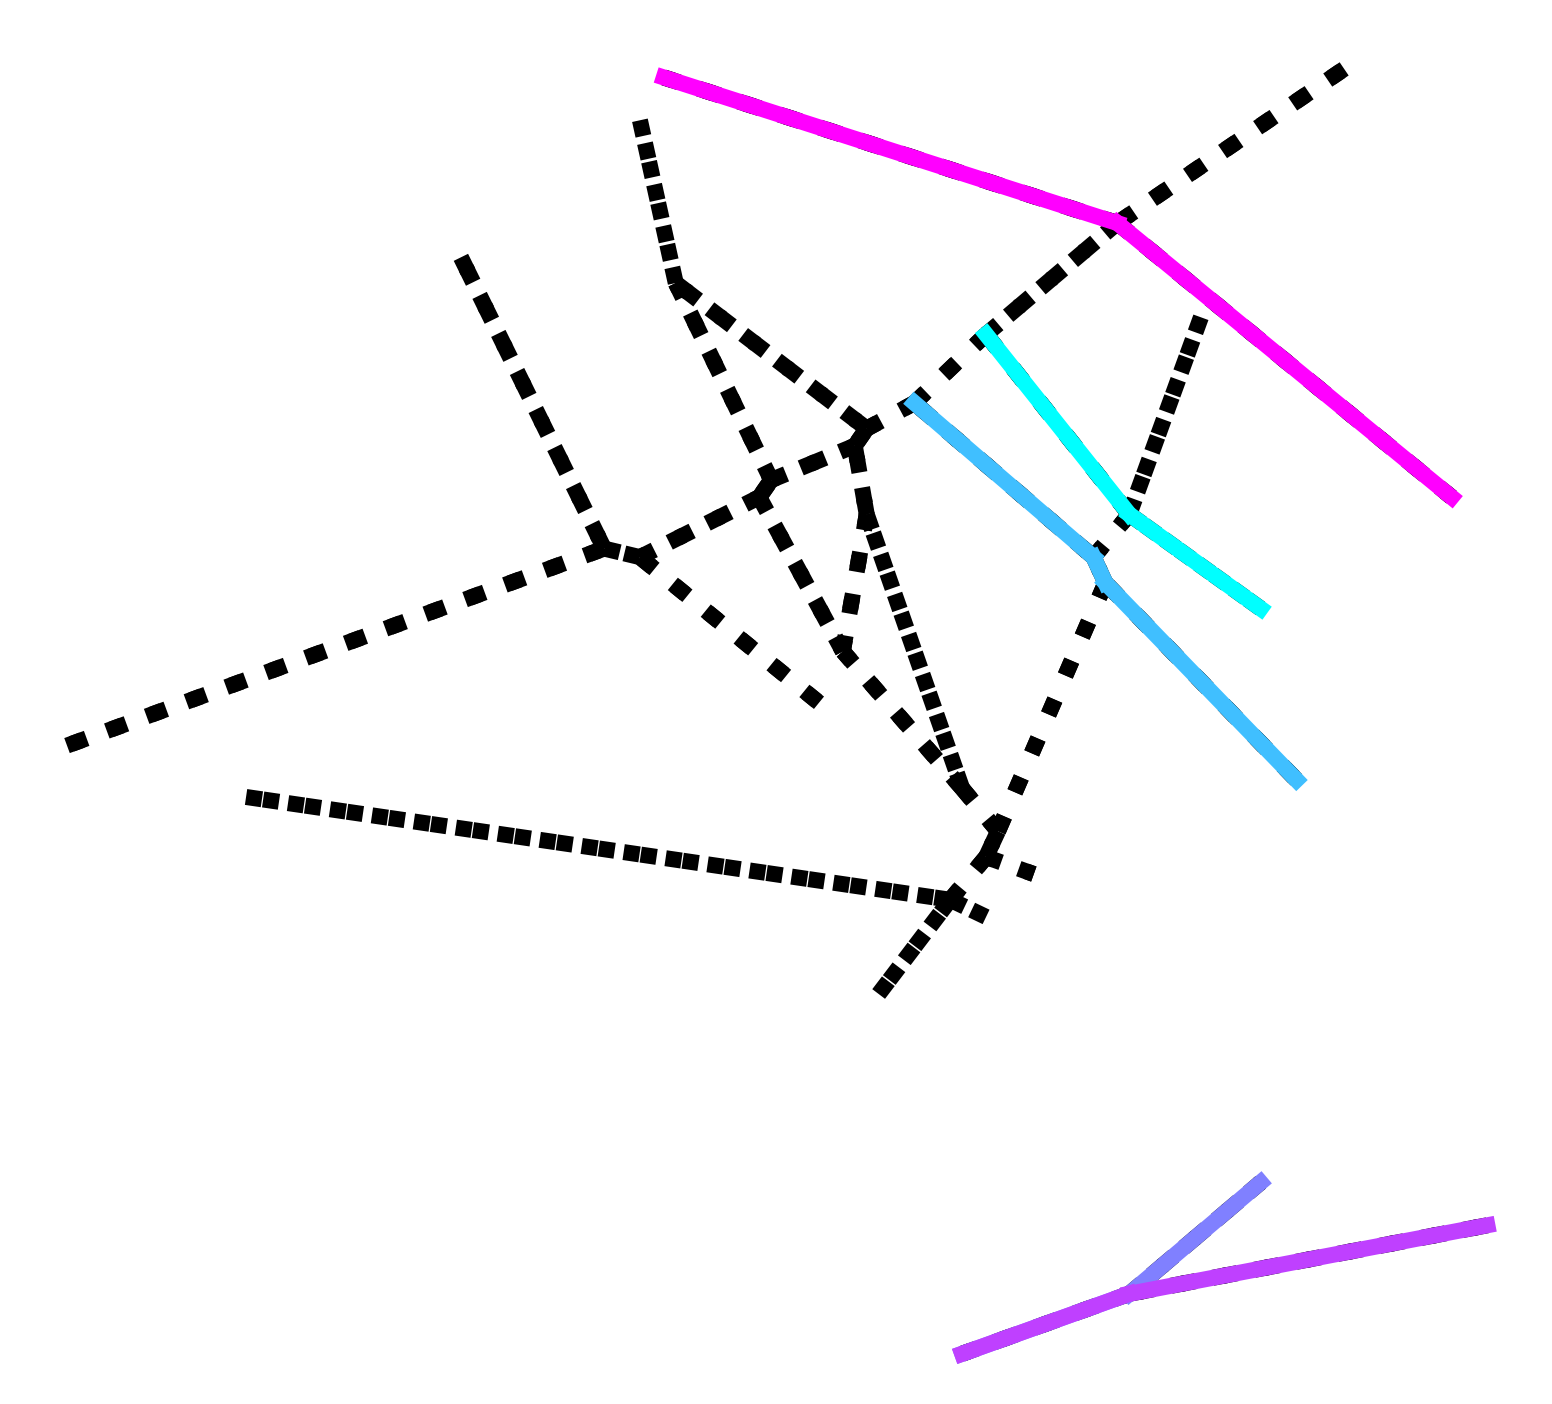
\includegraphics[height=1.5in]{resultImages/field3-t0-2cellBcrop-filtered-DeFiNeExactMatch-30.png}
        \caption{Filamentos correctamente individualizados por DeFiNe con 30\textdegree identificados con colores}
        \label{fig:field3t0filtered1Results-define30Exact}
    \end{subfigure}
    \vskip\baselineskip
    
    \begin{subfigure}[t]{0.49\textwidth}
        \centering
        \includegraphics[scale=0.6]{resultImages/field3-t0-2cellBcrop-filtered-DeFiNe60.png}
        \caption{Individualizaci\'on mediante DeFiNe con 60\textdegree}
        \label{fig:field3t0filtered1Results-define60}
    \end{subfigure}
    ~ 
    \begin{subfigure}[t]{0.49\textwidth}
        \centering
        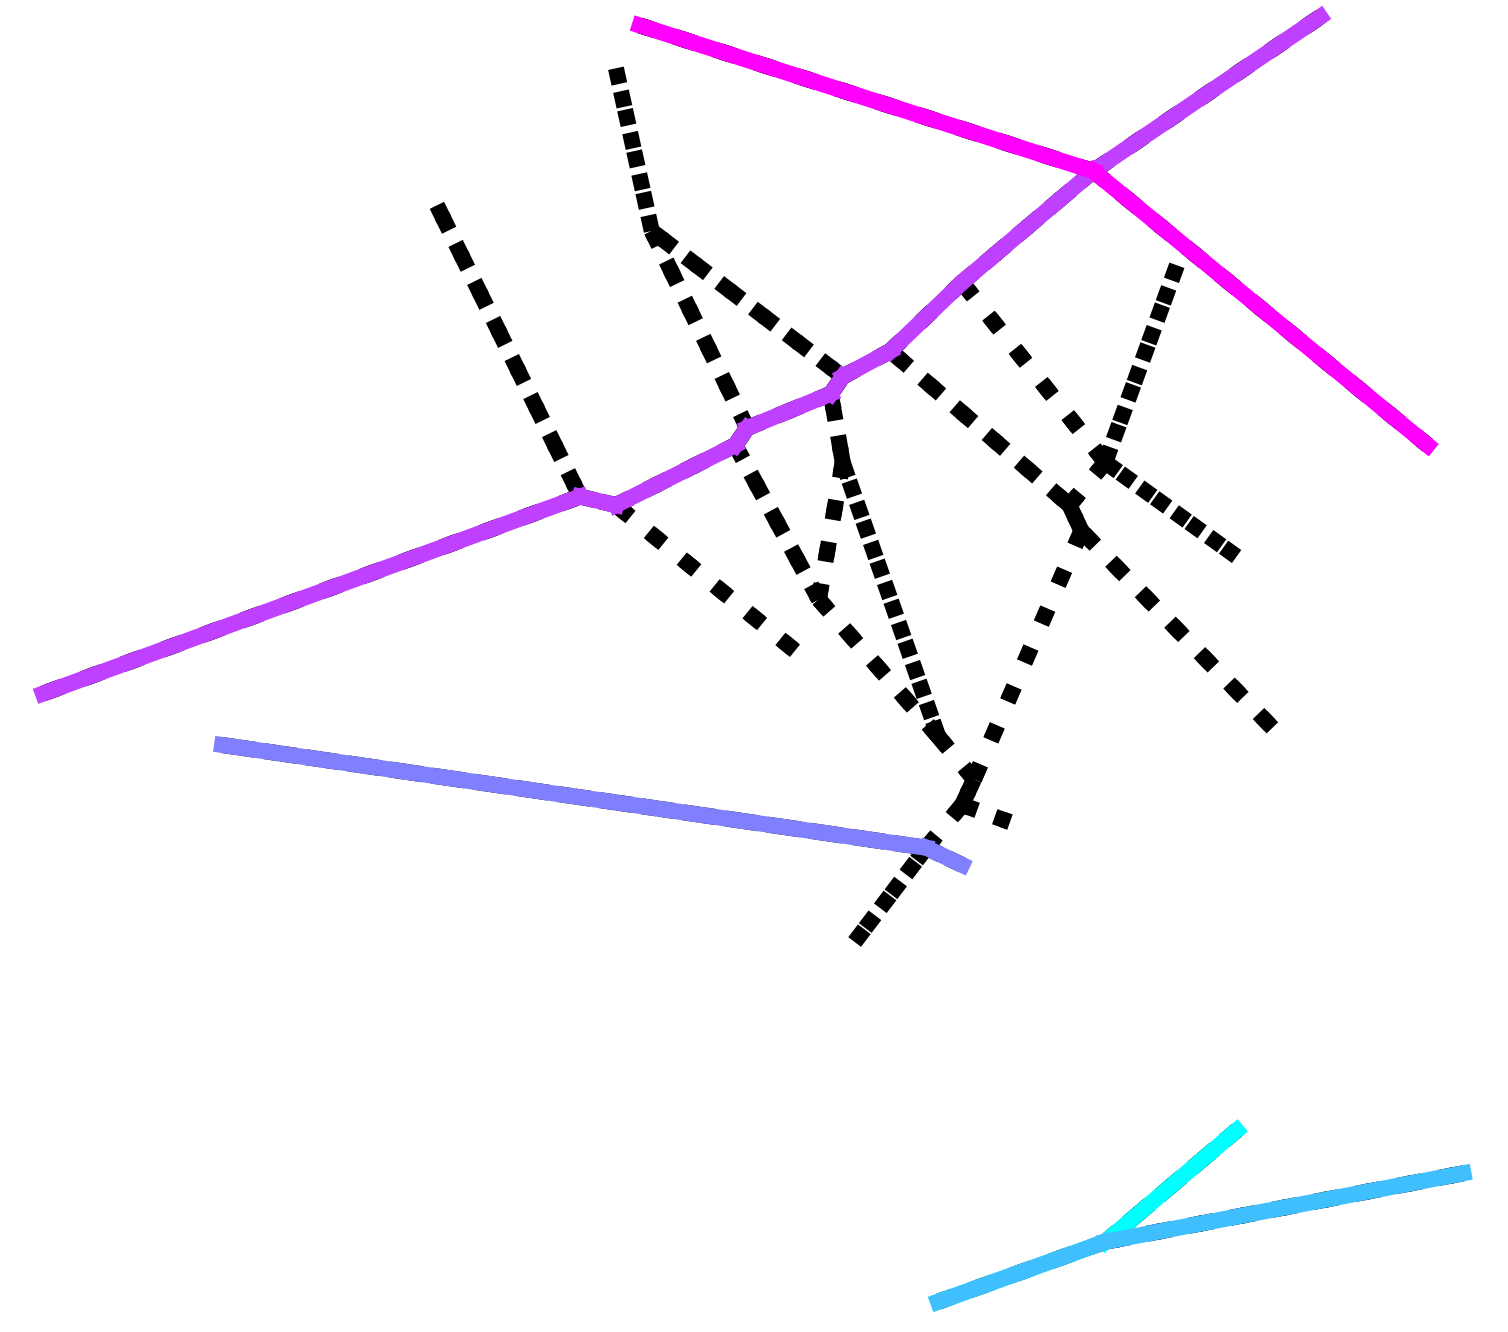
\includegraphics[height=1.5in]{resultImages/field3-t0-2cellBcrop-filtered-DeFiNeExactMatch-60.png}
        \caption{Filamentos correctamente individualizados por DeFiNe con 60\textdegree identificados con colores}
        \label{fig:field3t0filtered1Results-define60Exact}
    \end{subfigure}
    
    \vskip\baselineskip
    \begin{subfigure}[t]{0.49\textwidth}
        \centering
        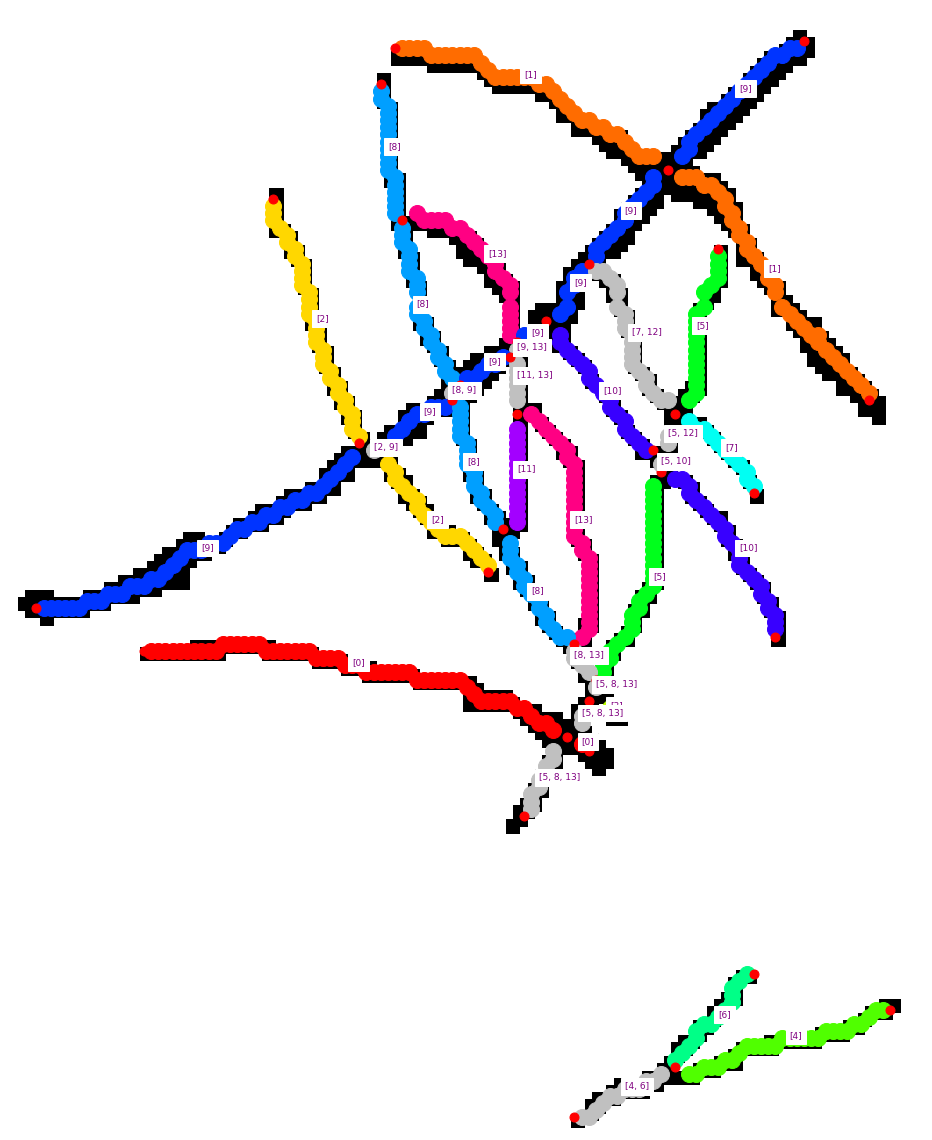
\includegraphics[height=1.5in]{resultImages/field3-t0-2cellBcrop-filtered-phil-s0-v05-antLabeled.png}
        \caption{Mejor Resultado de Individualizaci\'on con Phil}
        \label{field3t0filtered1Results-bestPhil}
    \end{subfigure}
    ~ 
    \begin{subfigure}[t]{0.49\textwidth}
        \centering
        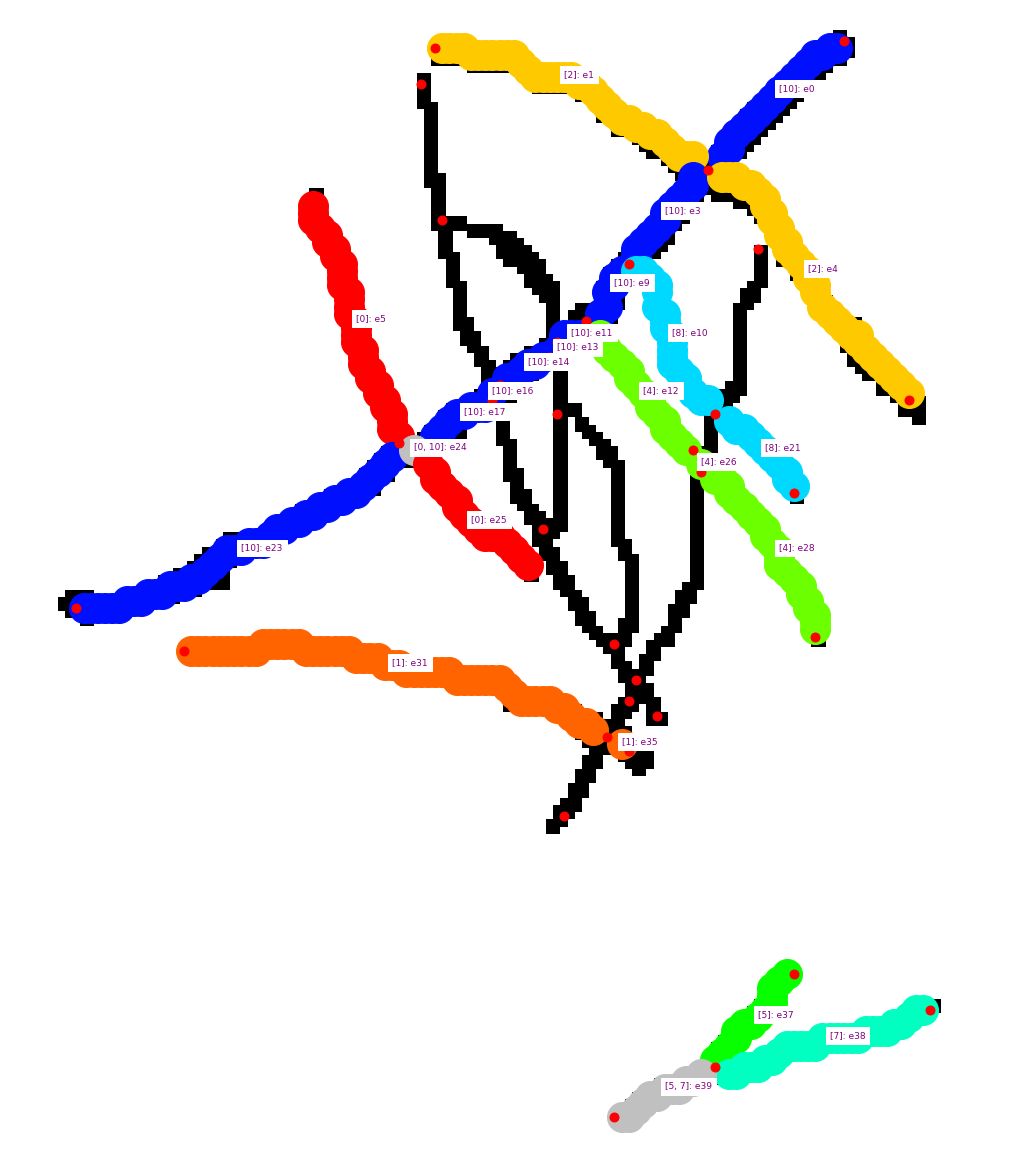
\includegraphics[height=1.5in]{resultImages/field3-t0-2cellBcrop-filtered-phil-s0-v05-exactMatch-antLabeled.png}
        \caption{Filamentos correctamente individualizados a partir del mejor resultado con Phil, identificados con colores}
        \label{fig:field3t0filtered1Results-bestPhilExact}
    \end{subfigure}
    \vskip\baselineskip
    
    \begin{subfigure}[t]{0.49\textwidth}
        \centering
        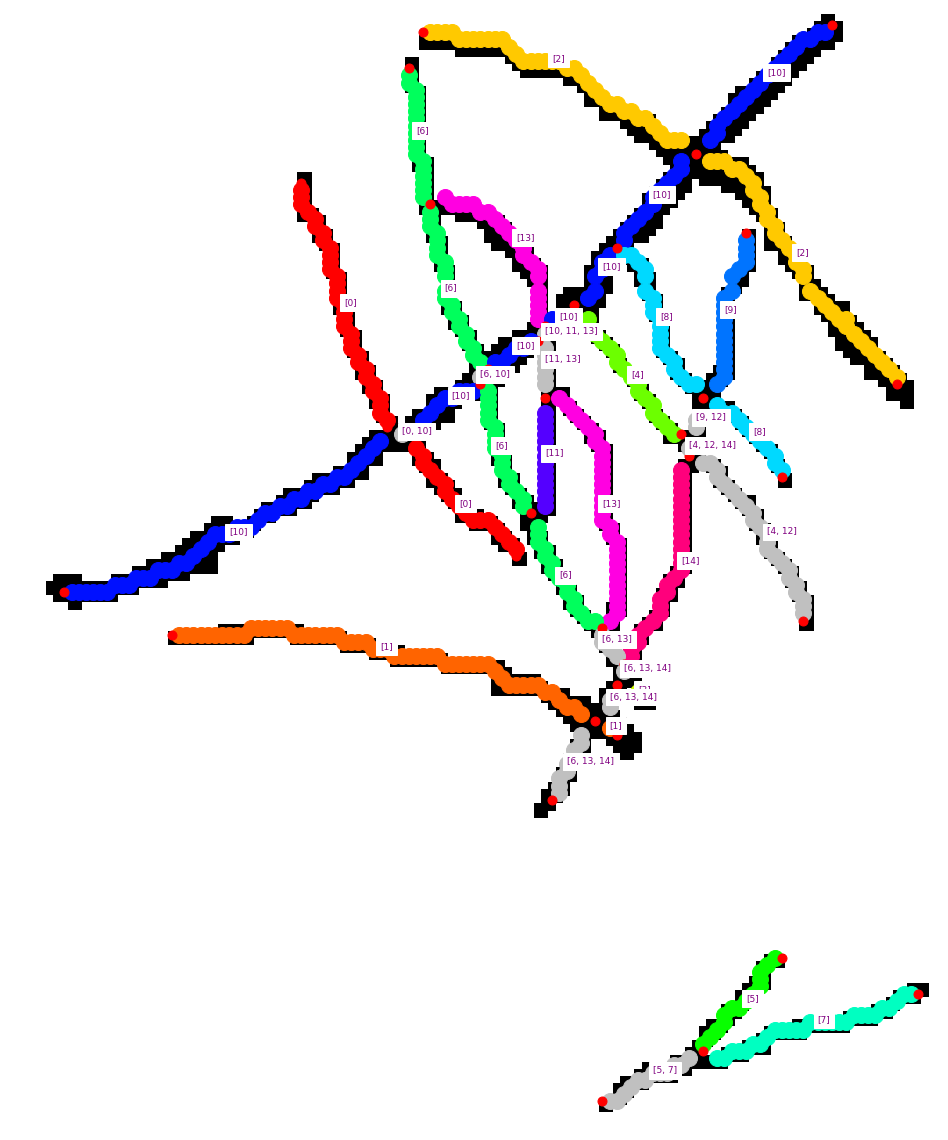
\includegraphics[height=1.5in]{resultImages/field3-t0-2cellBcrop-filtered-phil-s10-v05-antLabeled.png}
        \caption{Peor Resultado de Individualizaci\'on con Phil}
        \label{field3t0filtered1Results-worstPhil}
    \end{subfigure}
    ~ 
    \begin{subfigure}[t]{0.49\textwidth}
        \centering
        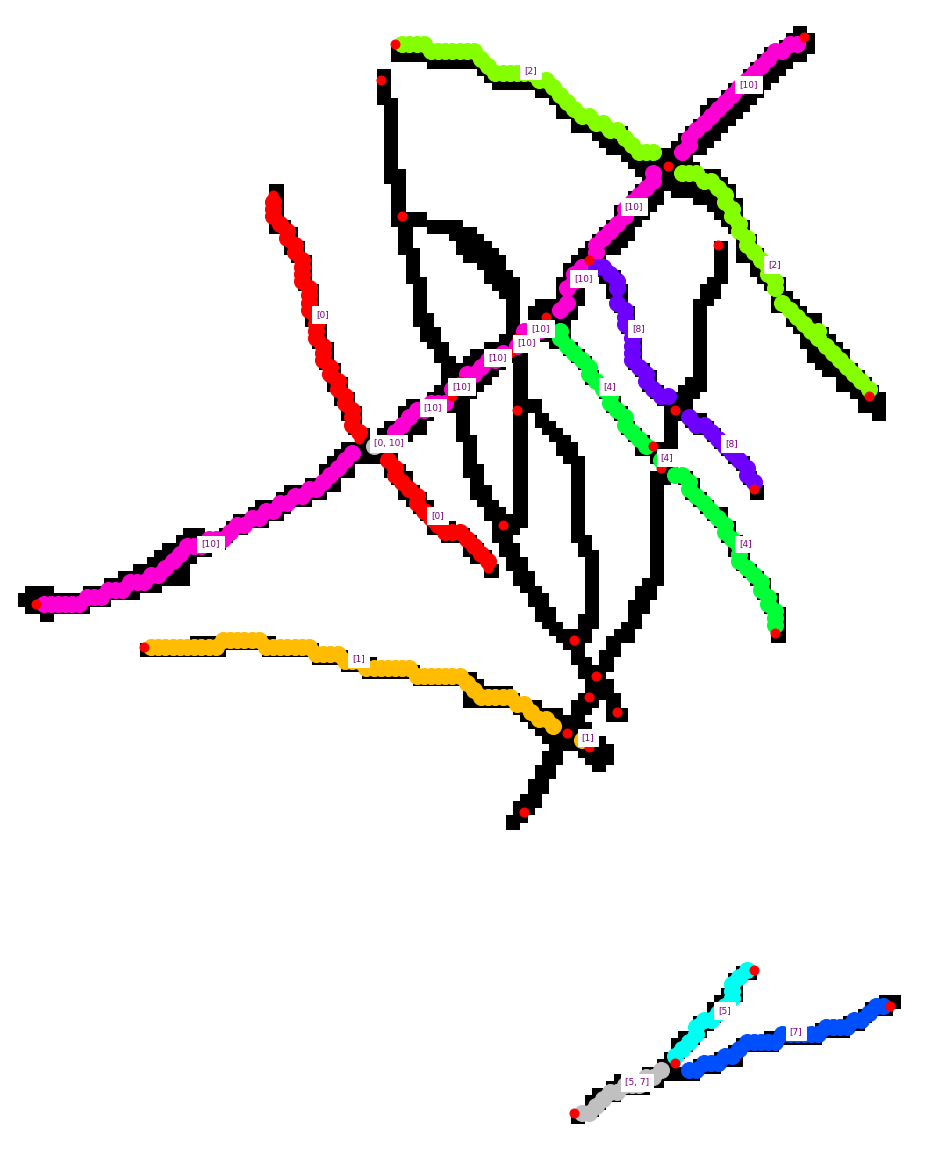
\includegraphics[height=1.5in]{resultImages/field3-t0-2cellBcrop-filtered-phil-s10-v05-exactMatch-antLabeled.png}
        \caption{Filamentos correctamente individualizados a partir del peor resultado con Phil, identificados con colores}
        \label{field3t0filtered1Results-worstPhilExact}
    \end{subfigure}
    
    \caption{Individualizaci\'on  de filamentos de la figura \ref{fig:field3t0filtered1} correspondiente a la muestra MT-B, realizadas con DeFiNe y Phil. Segmentos marcados en negro con y sin discontinuidad representan aristas no asignadas correctamente al filamento correspondiente en el {\it ground truth.}. f) El mejor resultado con Phil permite encontrar el filamento compuesto por las aristas 8,22,26,27,32,34,36 no encontrado en a) ni en c). }
    \label{fig:field3t0filtered1Results}
\end{figure*}

\begin{table}[h]
    \centering
    \begin{tabular}{|c|c|c|c|c|c|c|c|c|c|c|}
    \hline
        Algoritmo & VI & TP & FP &TN &FN & Rand	& Jaccard &	Precision &	Recall &	F1 \\ \hline
        Define 30° & 1.9654 & 100 & 90 & 1615 & 148 & 0.8781 & 0.2958 & 0.5263 & 0.4032 & 0.4566\\
        Define 60° & 1.8847 & 18 & 17 & 962 & 84 & 0.9065 & 0.1512 & 0.5142 & 0.1764 & 0.2627\\ 
        Phil & 2.3895 & 105.4 & 102.4 & 2028.4 & 224 & 0.8683 & 0.2487 & 0.5079 & 0.3283 & 0.3976 \\
        \hline
    \end{tabular}
    \caption{Resultados de individualizaci\'on de filamentos para la muestra MT-B (figura \ref{fig:field3t0filtered1}). El valor m\'aximo de VI en este caso es de 3.7612, ya que el tama\~no del {\it data set} es de 40 aristas. El n\'umero de filamentos en el {\it ground truth} es 12.}
    \label{tab:field3t0filtered1}
\end{table}
\addtocounter{table}{-1}
\begin{table}[h]
    \centering
    \begin{tabular}{|c|c|c|c|c|c|c|}
    \hline
         & \multirow{4}{2cm}{\centering \% Cobertura de Aristas} & \multirow{4}{2cm}{Filamentos Propuestos} & \multirow{4}{2cm}{Filamentos Correctos} & \multirow{4}{2.5cm}{\% Correctos vs Propuestos} & \multirow{4}{2.5cm}{\centering \% Correctos vs {\it Ground Truth}} & \multirow{4}{1.2cm}{\centering Tiempo [seg]} \\
         &  &  &  & & &  \\
        Algoritmo &  &  &  & & &  \\
        &  &  &  & & &  \\ \hline
        Define 30° & 100 & 23 & 5 & 21.7391 & 41.6667 & 5.0306 \\
        Define 60° & 100 & 16 & 5 & 31.25 & 41.6667 & 16.2042 \\ 
        Phil & 100 & 15 & 8.8 & 58.7738 & 73.3333 & 0.9693 \\
        \hline
    \end{tabular}
    \caption{Resultados ({\it Continuaci\'on}) de individualizaci\'on de filamentos para la muestra MT-B (figura \ref{fig:field3t0filtered1}). El n\'umero de filamentos en el {\it ground truth} es 12.}
    %\label{tab:field3t0filtered1-2}
\end{table}


%Valor m\'ax de VI para \ref{tab:field3t0filtered2} es 1.9459.
%N\'umero de filamentos en el {\it Ground Truth} de la figura field3t0 es 5.

La individualizaci\'on de filamentos para la figura \ref{fig:field3t0filtered2} que representa la muestra MT-C resulta en un empate entre Phil y la configuraci\'on de DeFiNe con 60\textdegree, encontrando 4 de 5 filamentos cada uno, mientras que DeFiNe con 30\textdegree como umbral encuentra s\'olo 3 de 5 filamentos. El filamento faltante en DeFiNe-60\textdegree es el que esta compuesto s\'olo por la arista 4 (figura \ref{fig:field3t0filtered2Results-d}), mientras que en DeFiNe-30\textdegree se lleva a cabo una asignaci\'on de las aristas 0-3 a un filamento, y de la arista 1 a otro, siendo la combinaci\'on correcta seleccionar la arista 0 por si sola y las aristas 3-1 en conjunto (figura \ref{fig:field3t0filtered2Results-e}). Similar a lo que realiza Phil, tambi\'en asignado las aristas 3-0 a un filamento, pero a su vez asignando correctamente las aristas 3-1 (figura \ref{fig:field3t0filtered2Results-f}).  A diferencia de otros resultados, se presenta un solo resultado para Phil ya que las 5 iteraciones arrojan el mismo resultado.


En el caso de Phil, la elecci\'on de las aristas 0-3 para formar un filamento se condice con el comportamiento del algoritmo en buscar caminos/filamentos de mayor longitud que cumplan con el criterio de rectitud. Por otra parte, este caso en un microt\'ubulo puede corresponder a la fusi\'on de 2 microt\'ubulos en uno, denominado {\tt Zippering}, o al nacimiento de un microt\'ubulo a partir de uno existente, llamado {\tt Nucleaci\'on}. Ambas situaciones requieren de informaci\'on adicional para diferenciarlas, como el grosor de los segmentos de filamentos y el \'angulo entre los segmentos de filamentos que se separan del segmento com\'un. La variaci\'on o continuidad del grosor y que el \'angulo mencionado se encuentre en un rango que var\'ia seg\'un el tipo de c\'elula son cr\'iticos para aclarar cual es el caso observado. 


\begin{figure*}[h!]
    \centering
    \begin{subfigure}[t]{0.3\textwidth}
        \centering
        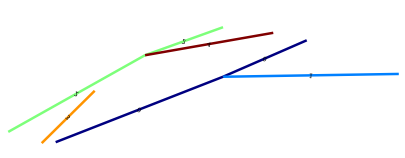
\includegraphics[scale=0.6]{resultImages/field3-t0-2cellBcrop-filtered-2-DeFiNe30.png}
        \caption{Individualizaci\'on mediante DeFiNe con 30\textdegree}
        \label{fig:field3t0filtered2Results-a}
    \end{subfigure}%
    ~ 
    \begin{subfigure}[t]{0.3\textwidth}
        \centering
        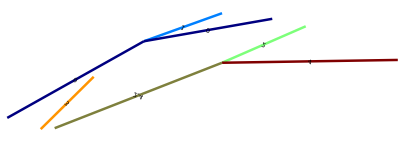
\includegraphics[scale=0.6]{resultImages/field3-t0-2cellBcrop-filtered-2-DeFiNe60.png}
        \caption{Individualizaci\'on mediante DeFiNe con 60\textdegree}
        \label{fig:field3t0filtered2Results-b}
    \end{subfigure}
    ~ 
    \begin{subfigure}[t]{0.3\textwidth}
        \centering
        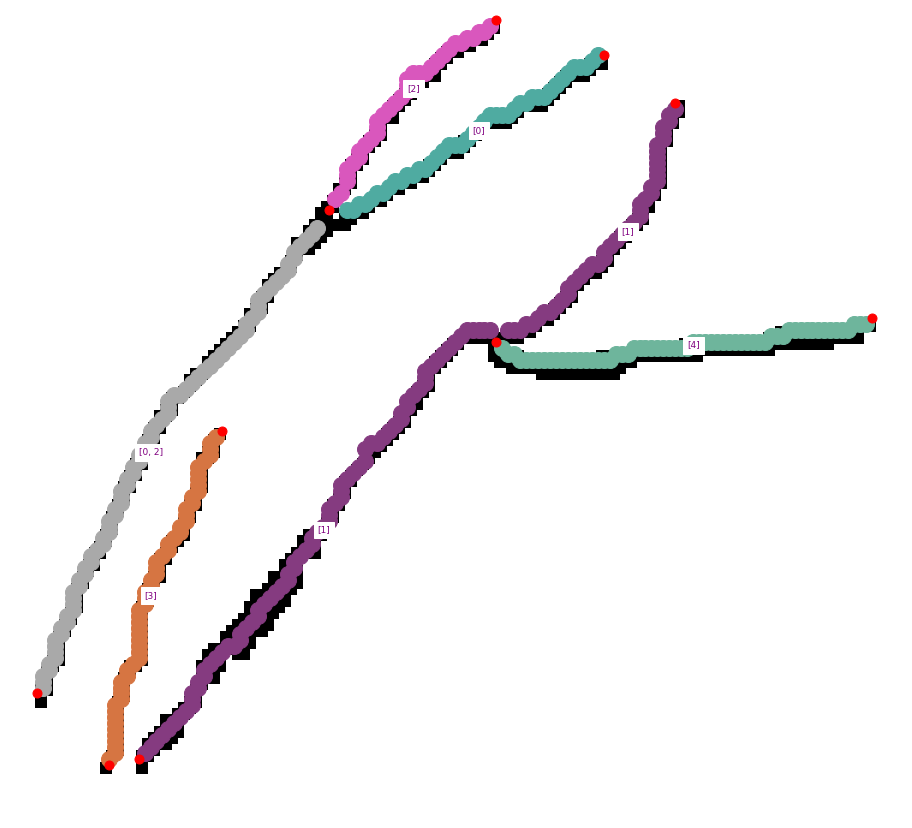
\includegraphics[height=1.5in]{resultImages/field3-t0-2cellBcrop-filtered-2-phil-s1271-v05-antLabeled.png}
        \caption{Individualizaci\'on con Phil}
        \label{fig:field3t0filtered2Results-c}
    \end{subfigure}
    \vskip\baselineskip
    
    \begin{subfigure}[t]{0.3\textwidth}
        \centering
        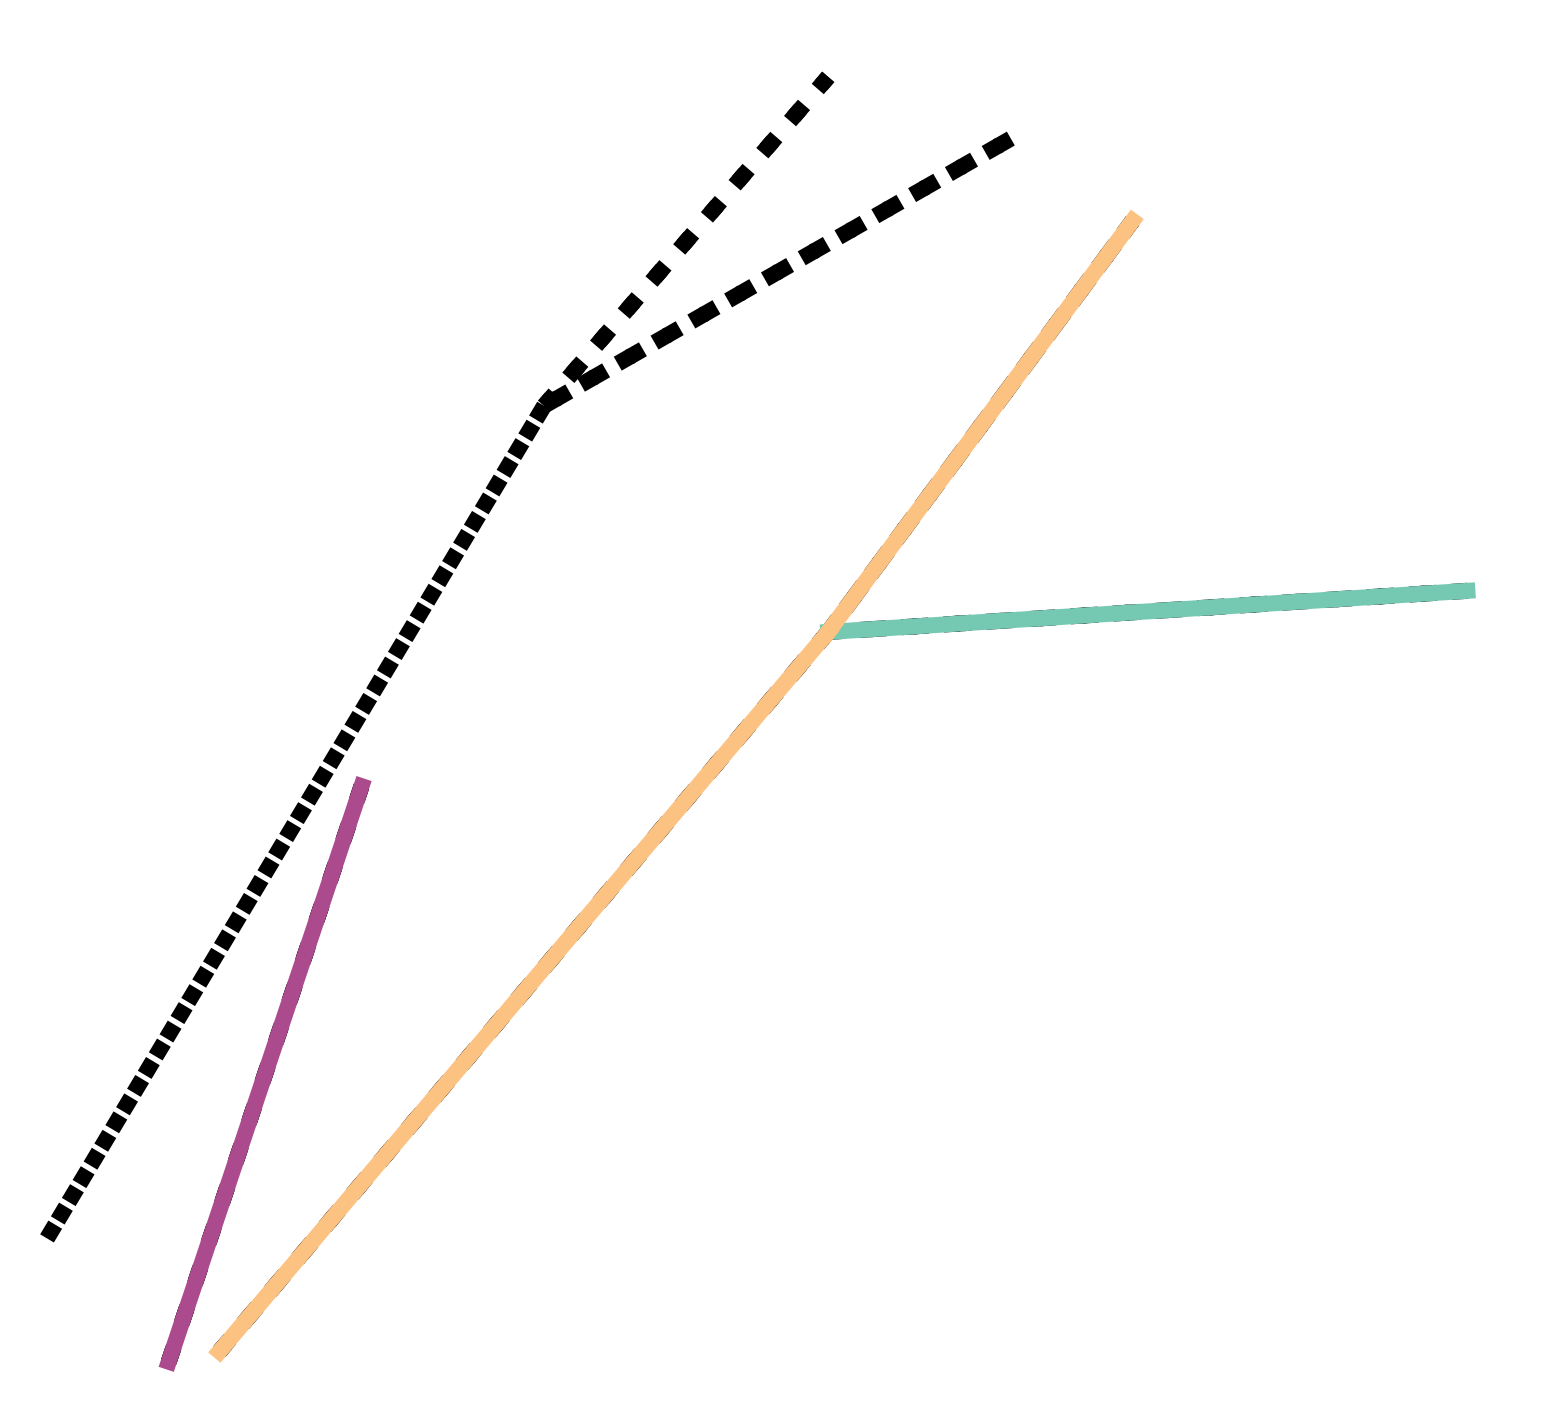
\includegraphics[height=1.5in]{resultImages/field3-t0-2cellBcrop-filtered-2-DeFiNeExactMatch-30.png}
        \caption{Filamentos correctamente individualizados por DeFiNe con 30\textdegree identificados con colores}
        \label{fig:field3t0filtered2Results-d}
    \end{subfigure}%
    ~ 
    \begin{subfigure}[t]{0.3\textwidth}
        \centering
        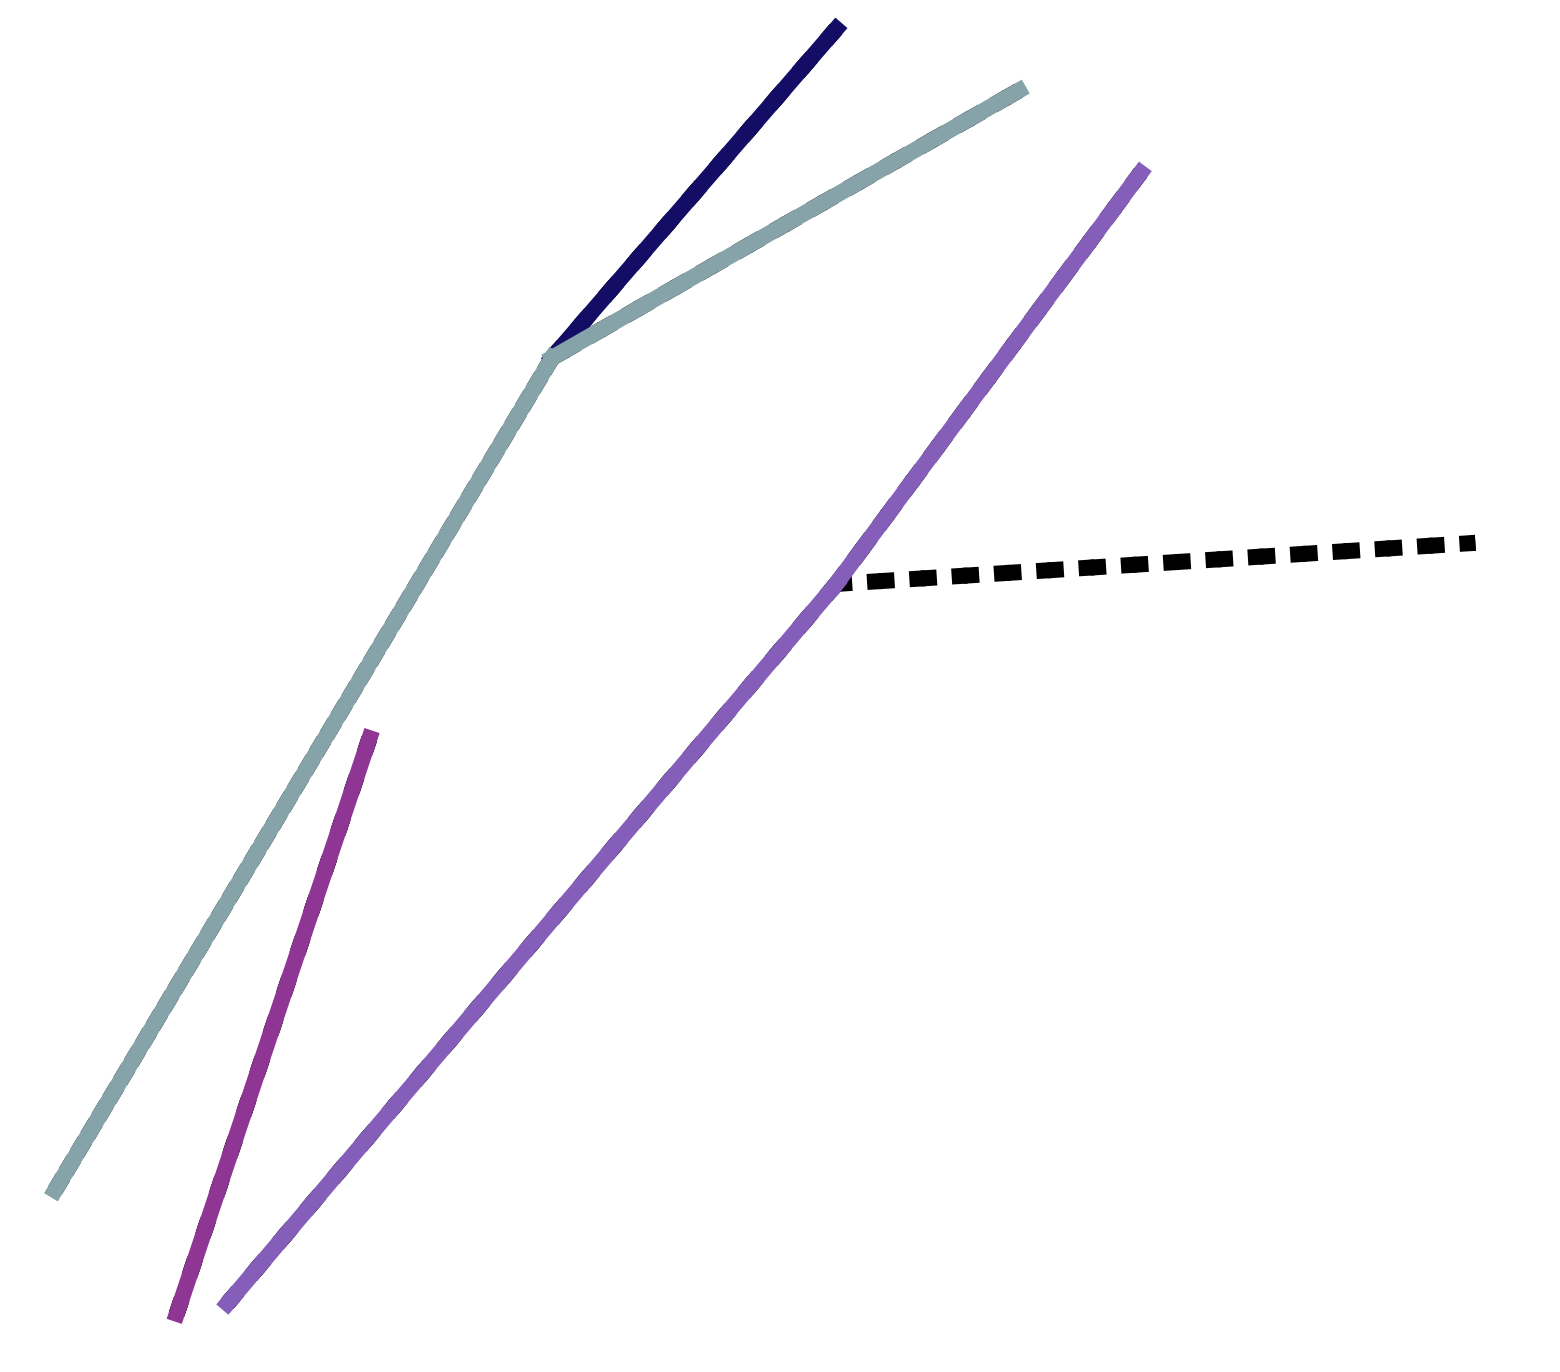
\includegraphics[height=1.5in]{resultImages/field3-t0-2cellBcrop-filtered-2-DeFiNeExactMatch-60.png}
        \caption{Filamentos correctamente individualizados por DeFiNe con 60\textdegree identificados con colores}
        \label{fig:field3t0filtered2Results-e}
    \end{subfigure}
    ~ 
    \begin{subfigure}[t]{0.3\textwidth}
        \centering
        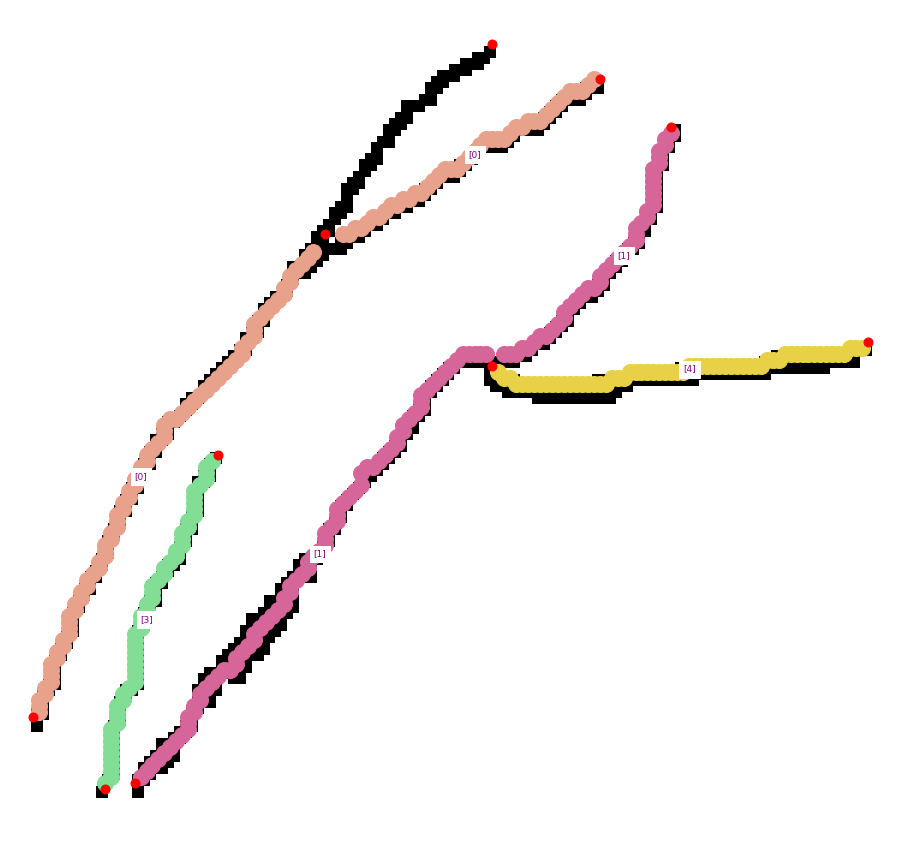
\includegraphics[height=1.5in]{resultImages/field3-t0-2cellBcrop-filtered-2-phil-s1271-v05-exactMatch-antLabeled.png}
        \caption{Filamentos correctamente individualizados por Phil identificados con colores}
        \label{fig:field3t0filtered2Results-f}
    \end{subfigure}
    
    \caption{Individualizaci\'on  de filamentos de la figura \ref{fig:field3t0filtered2} relativa a la muestra MT-C realizadas con DeFiNe y Phil. Segmentos marcados en negro con y sin discontinuidad representan aristas no asignadas correctamente al filamento correspondiente en el {\it ground truth.}.}
    \label{fig:field3t0filtered2Results}
\end{figure*}

En relaci\'on al an\'alisis de las medidas y las m\'etricas en la tabla \ref{tab:field3t0filtered2}, se mantiene el empate entre DeFiNe-60\textdegree y Phil, con la \'unica diferencia en el tiempo de ejecuci\'on, favorable para Phil. 

\begin{table}[h]
    \centering
    \begin{tabular}{|c|c|c|c|c|c|c|c|c|c|c|}
    \hline
        Algoritmo & VI & TP & FP &TN &FN & Rand	& Jaccard &	Precision &	Recall &	F1 \\ \hline
        Define 30° & 0.5714 & 1 & 1 & 18 & 1 & 0.9047 & 0.3333 & 0.5      & 0.5 & 0.5\\
        Define 60° & 0.4285 & 2 & 1 & 23 & 2 & 0.8928 & 0.4 & 0.6666 & 0.5 & 0.5714\\ 
        Phil & 0.4285  & 2 & 1 & 23 & 2 & 0.8928 & 0.4 & 0.6666 & 0.5 & 0.5714\\
        \hline
    \end{tabular}
    \caption{Resultados de individualizaci\'on de filamentos para figura \ref{fig:field3t0filtered2}, de la muestra MT-C. El valor m\'aximo de VI en este caso es de 1.9459, ya que el tama\~no del {\it data set} es de 7 aristas. El n\'umero de filamentos en el {\it ground truth} es 5.}
    \label{tab:field3t0filtered2}
\end{table}
\addtocounter{table}{-1}
\begin{table}[h]
    \centering
    \begin{tabular}{|c|c|c|c|c|c|c|}
    \hline
         & \multirow{4}{2cm}{\centering \% Cobertura de Aristas} & \multirow{4}{2cm}{Filamentos Propuestos} & \multirow{4}{2cm}{Filamentos Correctos} & \multirow{4}{2.5cm}{\% Correctos vs Propuestos} & \multirow{4}{2.5cm}{\centering \% Correctos vs {\it Ground Truth}} & \multirow{4}{1.2cm}{\centering Tiempo [seg]} \\
         &  &  &  & & &  \\
        Algoritmo &  &  &  & & &  \\
        &  &  &  & & &  \\ \hline
        Define 30° & 100 & 5 & 3 & 60 & 60 & 2.8262\\
        Define 60° & 100 & 5 & 4 & 80 & 80 & 2.6506\\ 
        Phil & 100 & 5 & 4 & 80 & 80 & 0.2914\\
        \hline
    \end{tabular}
    \caption{Resultados ({\it Continuaci\'on}) de individualizaci\'on de filamentos para figura \ref{fig:field3t0filtered2}, de la muestra MT-C. El n\'umero de filamentos en el {\it ground truth} es 5.}
\end{table}

\subsection{Neuronas}

\section{Resultados Generales}
t-test